% Created 2017-05-02 Tue 00:25
% Intended LaTeX compiler: xelatex
\documentclass[a4paper, notitlepage]{report}
\usepackage{graphicx}
\usepackage{grffile}
\usepackage{longtable}
\usepackage{wrapfig}
\usepackage{rotating}
\usepackage[normalem]{ulem}
\usepackage{amsmath}
\usepackage{textcomp}
\usepackage{amssymb}
\usepackage{capt-of}
\usepackage{hyperref}
% set the margins here, if they need to be modified
\usepackage[a4paper, left=1.3in, right=1.0in]{geometry}

\usepackage[style=ieee,backend=biber]{biblatex}

% The linespacing you want
\linespread{1.4}

% Lets you pick fonts. Only works if you compile with xelatex or luatex
\usepackage[no-math]{fontspec}

\usepackage{unicode-math}

\usepackage{stackengine}
\stackMath

% Used to make the captions on figures sans serif
\usepackage{caption}

% For including images
\usepackage{graphicx}
\usepackage{float}

\usepackage{color}

% For fancy code listings
\usepackage{minted}
\usemintedstyle{emacs}

% For tables that span multiple pages elegantly
\usepackage{longtable}

% For maintaining a list of abbreviations
\usepackage{nomencl}

% For drawing diagrams
\usepackage{tikz}

% These closely match the SCSS word template fonts
% Won't work unless you compile with xelatex or luatex
\setmainfont[Mapping=tex-text]{Times New Roman}
\setsansfont{Helvetica}
\setmonofont[Scale=MatchLowercase]{Monaco}
\setmathfont{TeX Gyre Termes Math}

\hypersetup{
  colorlinks,
  citecolor=black,
  filecolor=black,
  linkcolor=black,
  urlcolor=black
}

% Change these as appropriate, and they'll be filled in automatically on the
% cover page. You can also use them throughout the document, so as not to have
% to type them again all the time.
\newcommand \authorname{Eoin Houlihan}
\newcommand \authoremail{ehoulih@tcd.ie}
\newcommand \supervisorname{Dr. Glenn Strong}
\newcommand \degreetitle{B.A.(Mod.) Computer Science}
\newcommand \projecttitle{Dependent Types in Practice}

% All the commands are defined in this file
\newcommand \inserttitlepage{\thispagestyle{empty}
\begin{center}
{\sffamily
{\Large University of Dublin}

\vspace{10pt}


\includegraphics[scale=0.12]{tcd/trinitycollege.pdf}

\vspace{10pt}

{\Huge TRINITY COLLEGE}

\vspace{80pt}

\textbf{ \Large \emph \projecttitle}

\vspace{30pt}

\authorname

\degreetitle

Final Year Project May 2017

Supervisor: \supervisorname

\vspace{130pt}

\large{School of Computer Science and Statistics
\\$ $\\
O'Reilly Institute, Trinity College, Dublin 2, Ireland}
\linespread{1}
}
\end{center}
}
\newcommand \insertabstract{\begin{abstract}
\thispagestyle{plain}
Major software vulnerabilities in critical software have led to more interest in
formal verification of our software. One way that has presented itself to verify
our code is by using dependent types, an idea from the 1970s present in a number
of upcoming programming languages and interactive theorem provers.

We present a study into the current state-of-the-art dependently-typed
programming languages. Idris was chosen as the tool to carry out this study. The
methodology involved carrying out case studies of applying dependent types to
real-world programming problems. An evaluation of the outcomes and the current
landscape of dependently-typed programming languages applied in a practical
sense is provided as a result of carrying out these case studies.
\end{abstract}
}
\newcommand \declaration{\chapter*{Declaration}

I hereby declare that this project is entirely my own work and that it has not
been submitted as an exercise for a degree at this or any other university.
$ $\\
$ $\\
\signed{\authorname}
}
\newcommand \acknowledgements{\chapter*{Acknowledgements}
Firstly, I would like to thank my parents for giving me the opportunity, support
and encouragement I needed throughout my degree.

\noindent
I would like to thank Glenn Strong for his continued guidance and suggestions
throughout this project as my supervisor.

\noindent
I would also like to thank the budding Idris and dependent type community,
particularly those in the \#idris IRC channel, for being patient enough to
answer any questions that I had.
}
\newcommand \permissiontolend{\chapter*{Permission to lend}

I agree that the Library and other agents of the College may lend or copy
this report upon request.

$ $\\
$ $\\
\signed{\authorname}
}
\newcommand \ibidp{(\emph{Ibid.})}
\newcommand \ibid{\emph{Ibid.}}

\newcommand{\argmax}[1]{\underset{#1}{\operatorname{arg}\,\operatorname{max}}\;}

\usepackage{datetime}

\def\fullhrulefill{\leavevmode\leaders\hrule height 1pt\hfill\kern 0pt}

\newcommand{\signedanddate} {
  \par\noindent\makebox[2.5in]{\fullhrulefill}
  \par\noindent\makebox[2.5in][l]{\authorname, May 5 2017}
}

\newcommand \needcite[1]{\underline{#1}}

\newcommand \abbrev[2]{#1\nomenclature{#1}{#2}}


% For changing the names of the List of Listings, etc.
\renewcommand*{\contentsname}{Table of Contents}
\renewcommand*{\nomname}{Abbreviations}

% Make the captions sans serif
\renewcommand{\captionfont}{\sffamily}

\addbibresource{report.bib}
\author{Eoin Houlihan}
\date{\today}
\title{Dependent Types in Practice}
\hypersetup{
 pdfauthor={Eoin Houlihan},
 pdftitle={Dependent Types in Practice},
 pdfkeywords={},
 pdfsubject={},
 pdfcreator={Emacs 25.2.1 (Org mode 9.0.5)},
 pdflang={English}}
\begin{document}

\inserttitlepage
\pagenumbering{roman}
\declaration
\permissiontolend
\insertabstract
\acknowledgements
\tableofcontents
\newpage
\pagestyle{headings}
\pagenumbering{arabic}

\chapter{Introduction}
\label{sec:org0fffd94}
\begin{quote}
``Beware of bugs in the above code; I have only proved it correct, not tried
it.''

-- Donald Knuth
\end{quote}

Software now more than ever plays an important role in the management of
critical infrastructure such as our railways, hospitals and the internet.
Critical software vulnerabilities such as the Heartbleed \cite{heartbleed_2014}
bug in OpenSSL expose us to the perils of poorly specified and incorrect
software. In the case of Heartbleed this meant that important cryptographic keys
and secrets were leaked over the internet due to a memory access bug.

Formal verification of software has seen an increase in interest in recent years
due to bugs such as this. Dependent types offer us a way to formally verify code
by stating correctness properties in the types of our functions and data types.
Any type-checked implementation of these functions serves as a proof that these
properties hold in our code.

\begin{center}

\includegraphics[width=0.35\linewidth]{./fig/heartbleed.png}
\end{center}

The aim of this project is to evaluate the practical usage of state-of-the-art
dependently-typed programming languages. We will choose to use Idris in
particular as the tool to work with. The evaluation of a key set of objectives
will take place following the implementation of case studies of real-world
programs. These programs have been written while taking advantage of correctness
properties and dependent types to ensure a more rigorous and correct program
than one written using a conventional programming language.

\section{Report Structure}
\label{sec:org232eb67}
The remainder of this report is structured as follows:
\begin{itemize}
\item \emph{Chapter 2} provides the necessary background information about the theory and
logic behind dependent types as well as a look at the landscape of current
state-of-the-art dependently-typed programming languages.
\item \emph{Chapter 3} explains in more detail the project objectives and the approach
taken to complete these objectives.
\item \emph{Chapter 4} gives a detailed look into Idris both in terms of the syntax and
language features as well as the tooling and development methods used.
\item \emph{Chapter 5} is an examination of the implementation of the case studies carried
out in this project.
\item \emph{Chapter 6} details our conclusions and assessments having carried out the case
studies and evaluated the current landscape of dependent types.
\item \emph{Chapter 7} lists some possible areas of future work.
\end{itemize}
\chapter{Background}
\label{sec:orgb767833}
This chapter aims to give an understanding of the background and necessary
concepts that will be used throughout the report. A basic understanding of
functional programming ideas such as algebraic data types, recursion and the
fundamentals of the Hindley-Milner type system with respect to languages such as
Haskell is assumed of the reader. It also gives a broad overview of the current
state of the art dependently-typed programming languages with a more in-depth
look at Idris in particular.

\section{Intuitionistic Type Theory}
\label{sec:orgb6ac62a}
Intuitionistic type theory is a type theory based on mathematical
constructivism. Constructive mathematics is an alternative foundational theory
of mathematics that argues that construction of a mathematical object is
necessary to proving that such an object exists. Of particular note, the
intuitionistic logic which much of constructivism uses deviates from classical
logic systems in that proof by contradiction is not used and the law of the
excluded middle is not assumed as an axiom of the logic in general.

Drawing upon these ideas, Per Martin-Löf, a Swedish logician, developed a number
of successive type theories in the 1970s \cite{martin-lof_intuitionistic_1984}.
This intuitionistic type theory (also commonly referred to as Martin-Löf type
theory) introduces a number of interesting concepts. Most notable in terms of
their influences on programming language design were the concepts of \(\Pi\)-types
and \(\Sigma\)-types. These constructs can be seen as analogous to the logical
quantifiers ``forall'' and ``exists'' respectively. These concepts have served
as the underpinning of the development of dependently-typed programming
languages and theorem provers based on Martin-Löf type theory.

\section{Curry-Howard Isomorphism}
\label{sec:org8d3b9cc}
From a modern computer science perspective it's almost taken for granted that
computability theory and mathematical proofs are inherently linked. For example,
many parallels can be drawn between the proof of Turing's Halting Problem and
Gödel's incompleteness theorems. Between the 1930s and the 1960s Haskell Curry
and William Alvin Howard began to formalise this direct link between computer
programs and mathematical proofs which is known as the Curry-Howard isomorphism
\cite{mcadams_tutor_2013}. As Philip Wadler, one of the original authors of the
Haskell report, put it \cite{strange_loop_2015,wadler_propos_2015}

\begin{quote}
``Every good idea will be discovered twice. Once by a logician and once by a
computer scientist.''

-- Philip Wadler
\end{quote}

According to the Curry-Howard isomorphism the type of an expression is
equivalent to a proposition of a logical formula. A term inhabiting that type is
therefore equivalent to a proof that the proposition holds. Some concrete value
exists that bears witness to the type being inhabited. In other words, a proof
can be constructed. This very much aligns with the constructivist view of
mathematics. Other correspondences can be shown such as between logical
implication and function types, conjunction and product types and between false
formulas and the uninhabited type, bottom (\(\bot\)). We can even see from the
shape of the syntax rules of both natural deduction and simply-typed lambda
calculus that these kinds of correspondences exist. As an example, the
relationship between the Modus Ponens rule and the function application rule.
\[ \scalebox{2}{$\frac{\Gamma \vdash \alpha \rightarrow \beta \qquad \Gamma
\vdash \alpha}{\Gamma \vdash \beta} \rightarrow E \qquad \frac{\Gamma \vdash
t:\alpha \rightarrow \beta \qquad \Gamma \vdash u:\alpha}{\Gamma \vdash
t\;u:\beta}$} \]

One of the consequences of this relationship is the possibility of a unification
at a primitive level between mathematical logic and the foundations of
computation. In practical terms this relationship has influenced the work on
programming languages such as Coq and Idris that allow proofs to be written as
programs that can be formalised, verified and executed. This is interesting to
the practice of software engineering as it gives us the power to reason about
program correctness by translating a mathematical proof of an algorithm to a
computer program and having the machine type-check (proof-check) it.

\section{Traditional Hindley-Milner Type Systems}
\label{sec:org04b2771}
Standard Hindley-Milner-esque type systems such as the one found in Haskell
allow us to express some different dependencies between the types of terms and
terms themselves. For example, terms can depend on other terms such as in this
Haskell function definition.

\begin{listing}[H]
\begin{minted}[frame=single,fontsize=\normalsize,linenos,breaklines,escapeinside=\#\#]{haskell}
plusOne x = x + 1
\end{minted}
\caption{A simple Haskell function definition (terms depending on terms)}
\end{listing}

Here we can see that the term \texttt{plusOne} has been defined with respect to the
terms \texttt{x}, which is its argument and \texttt{1}, an integer. Types can also depend on
other types as shown here.

\begin{listing}[H]
\begin{minted}[frame=single,fontsize=\normalsize,linenos,breaklines,escapeinside=\#\#]{haskell}
data List a = Nil
            | Cons a (List a)
\end{minted}
\caption{A Haskell data type definition with a type parameter (types depending on types)}
\end{listing}

In this Haskell data type definition, the type constructor \texttt{List} depends on the
type \texttt{a} provided to it. This allows polymorphism and lists of any type.
Finally, in the world of Haskell, terms can depend on types. This is apparent in
polymorphic functions such as the identity function.

\begin{listing}[H]
\begin{minted}[frame=single,fontsize=\normalsize,linenos,breaklines,escapeinside=\#\#]{haskell}
id :: a -> a
id x = x
\end{minted}
\caption{A polymorphic Haskell function definition (terms depending on types)}
\end{listing}

\section{Dependent Type Systems}
\label{sec:orge67bb1b}
Dependent type systems extend this system of dependencies by allowing types to
depend on terms. This leads to much greater expressivity power in the type
system. For example, in a dependently typed system we can express types such as
the type of pairs of natural numbers where the second number is greater than the
first.

If we take the view of the Curry-Howard isomorphism that types are propositions
and terms are witnesses to a proof of that proposition then we can see the
advantages of a more expressive type system. We can now encode much more
sophisticated propositions in the type system and if we can prove them (i.e.
construct a value that inhabits that type) then we can guarantee much more
interesting correctness properties about the code that we are writing. For this
reason, dependent types have seen much use in the areas of formal verification
of computer programs and formal computer encoding of mathematical objects and
proofs.

There are 3 main concepts taken from Martin-Löf type theory and implemented in
dependently-typed programming languages.

\subsection{\texorpdfstring{$\Pi$}{Pi}-types}
\label{sec:orgdca1296}
\(\Pi\)-types are the types of functions whose return types depend on one or more of
their arguments. In other words these functions map values from some domain to
some non-fixed codomain that is determined by the input. In this sense the
return type is said to be dependent upon the input.

If we have a representation of \(n\textrm{-tuples}\) of some type \(A\),
\(\operatorname{Vect}(A,n)\), then the \(\Pi\)-type \(\Pi_{(n \mathbin{:} {\mathbb N})}
\operatorname{Vect}(A,n)\) represents the type of functions that given some
natural number \(n\) return a tuple of size \(n\) of elements of type \(A\). That is
to say that the type of the value returned by these functions is determined by
the argument to the functions.

\subsection{\texorpdfstring{$\Sigma$}{Sigma}-types}
\label{sec:org3765d17}
\(\Sigma\)-types, also known as dependent pair types, are a more generalised form of
Cartesian product that model pairs of values where the type of the second
element depends on the first element.

Again using the \(\operatorname{Vect}\) representation of \(n\textrm{-tuples}\) of
some type \(A\), the \(\Sigma\)-type \(\Sigma_{(n \mathbin{:} {\mathbb N})}
\operatorname{Vect}(A,n)\) represents a pair of a natural number \(n\) and a tuple
of length \(n\) of values of type \(A\).

This representation is similar to the Haskell \texttt{List} type however there is extra
information in that the type of the \(\Sigma\)-type \(\operatorname{Vect}\) also
carries around a witness to its length expressed as a natural number. We say
that \(\operatorname{Vect}\) is ``indexed'' by the type \(A\) as well as the value
\(n\).

Being able to index types by both types and terms in the language is a key
feature of dependently-typed programming languages. These languages eliminate
the distinction between types and terms. Types and terms are unified as
equivalent constructs.

\subsection{The Equality Type}
\label{sec:org18d4c71}
The equality type \(=\) is a special type used to denote proofs of equality
between two values. If there is an inhabitant of the type \(a \mathrel{=} b\) then
\(a\) and \(b\) are considered to be equal. This proof allows \(b\) to be used
anywhere \(a\) would have been used. There is only one inhabitant of the type \(a
\mathrel{=} a\), the reflexive proof of equality.

\[ \scalebox{2}{$\operatorname{refl} \mathbin{:} \Pi_{(a \mathbin{:} A)} (a
\mathrel{=} a)$} \]

This type is particularly useful in dependently-typed programming in that it can
be used as a witness that two terms are equivalent and allows a substitution of
one term for another to take place. With it, we can begin to develop
constructions of basic proofs and axioms such as \(n \mathbin{:} {\mathbb N}, n
\mathbin{-} n \mathrel{=} 0\).

\section{State of The Art Dependently-Typed Programming Languages}
\label{sec:org7b5319d}
\subsection{Agda}
\label{sec:org3d407e5}
Originally developed in the late 1990s by Catarina Coquand and subsequently
rewritten by Ulf Norell in 2007, Agda is a dependently typed programming
language with support for features such as dependent pattern matching and
definition of inductive data types.

For example, the inductive data type representing the Peano natural numbers can
be declared as follows in Agda.

\begin{listing}[H]
\begin{minted}[frame=single,fontsize=\normalsize,linenos,breaklines,escapeinside=\#\#]{agda}
data #$ℕ$# : Set where
  zero : #$ℕ$#
  suc : #$ℕ$# → #$ℕ$#
\end{minted}
\caption{Agda definition of a natural number type}
\end{listing}

There are two cases to consider here. \texttt{zero} is the base case. \texttt{suc} (standing
for successor) takes a natural number and returns a new natural number. It
represents a natural number plus 1. We will see more definitions of inductive
types similar to this one throughout the later chapters.

Agda has the capability of producing executable code however it is mostly used
for the purpose of automated theorem proving. Agda does however provide a
foreign function interface to import arbitrary Haskell types and functions.
These go unused for the purpose of Agda type-checking but do have runtime
effects in the output compiled code.

\subsection{Coq}
\label{sec:orgad43672}
Developed initially in the late 1980s at INRIA in France, Coq approaches
dependently-typed programming more from the mathematical side as an interactive
theorem prover. Coq is based on the Calculus of Constructions, a type theory
created by Thierry Coquand. Coq provides useful facilities for defining
inductive data types and includes a tactics language for doing interactive
proofs.

Notable work created using Coq includes the formally verified C compiler
CompCert \cite{leroy_compiler_2009}, as well as a formally verified proof of the
Four-Colour Theorem \cite{gonthier_formal_2008} for graph colouring.

Development in Coq and using dependent types in general can become quite
complex. To support the powerful type system a number of featureful interactive
environments such as CoqIDE and Proof General \cite{proof_general} exist. These
environments provide semantic information about your code. This includes the
current environment of defined values as well as their types and the type of the
current goal that you are attempting to prove.

\begin{figure}[H]
\centering
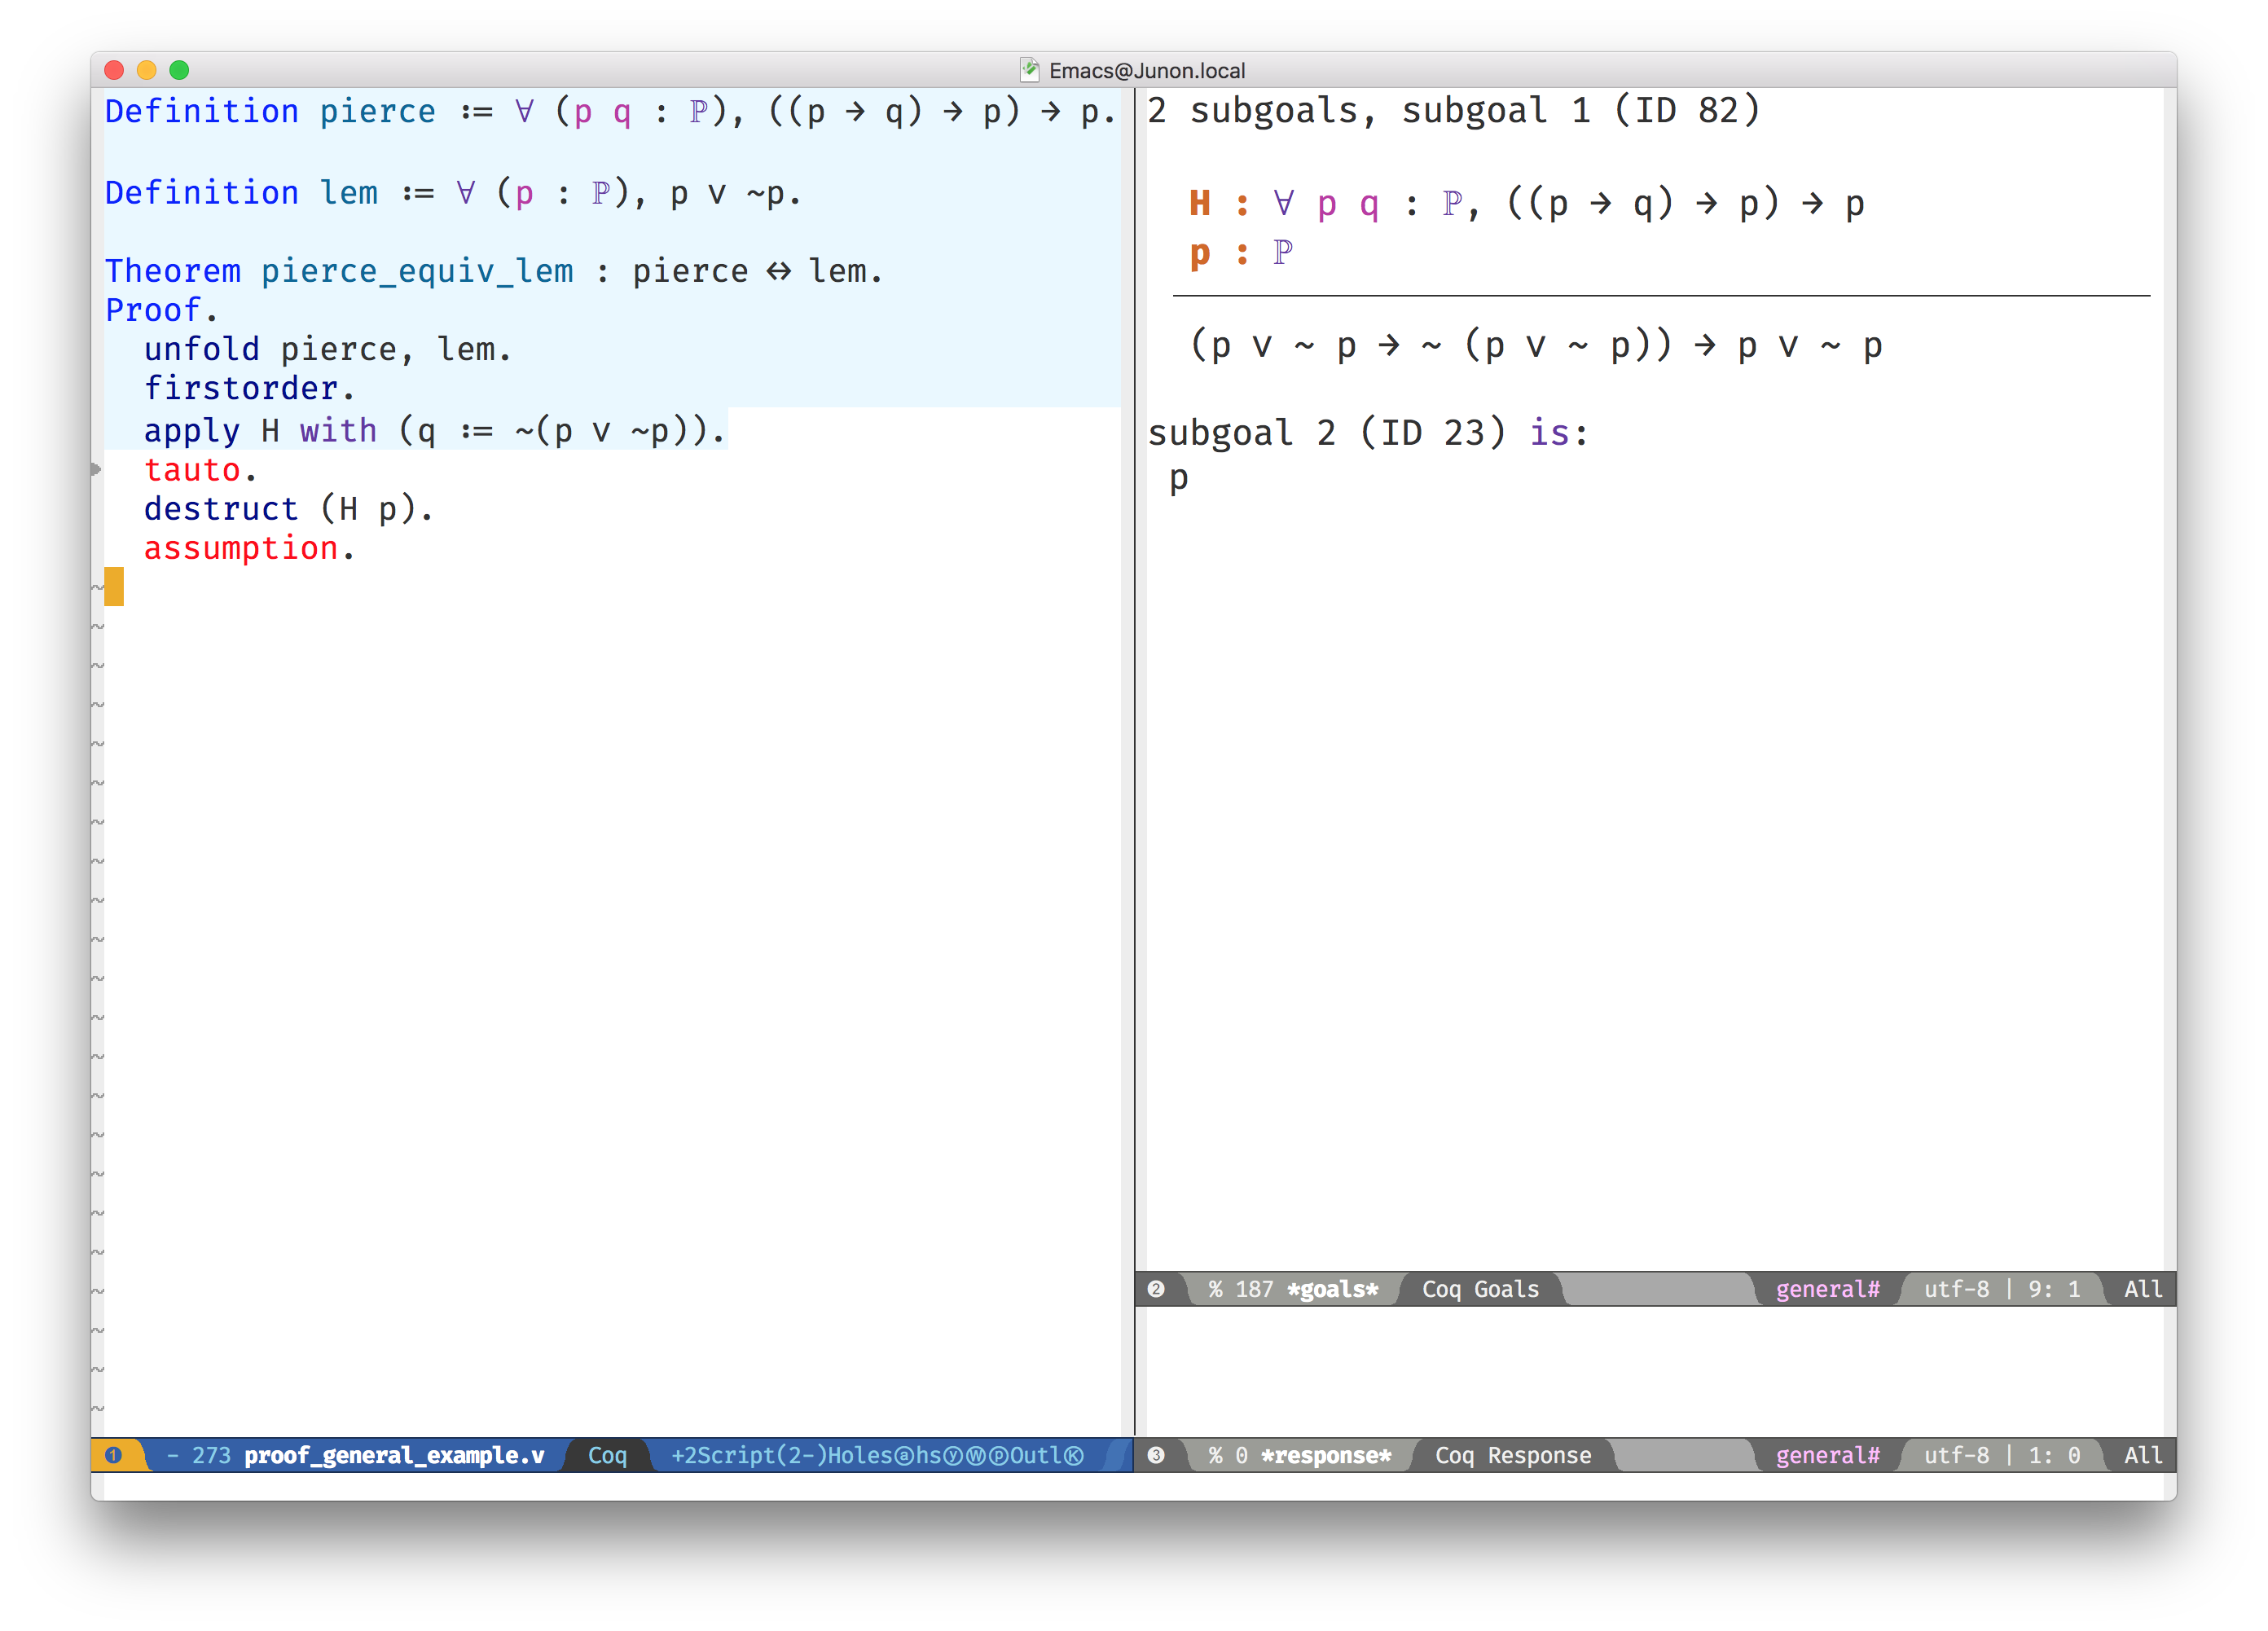
\includegraphics[width=0.85\linewidth]{./fig/proof_general.png}
\caption{An in-progress Proof General session}
\end{figure}

Coq's primary mechanism for producing executable code is via program extraction.
This is the process by which correct Coq code can be transformed into an
equivalent Haskell or OCaml module which provides the user with the ability to
run the extracted code. This extraction process has benefits in that it allows
for the expression and type-checking of interesting correctness properties in a
dependently-typed language while also giving us a way to compile it to native
code using compilers with state-of-the-art code optimisation techniques. This
allows the production of a fast native binary from a correct and type-checked
Coq program.

\subsection{Haskell}
\label{sec:org3da022b}
GHC Haskell has slowly been implementing many of the capabilities of dependent
types via extensions to the language such as \texttt{GADTs}, \texttt{DataKinds}, and
\texttt{TypeFamilies}. Through particular use of the Haskell type system many of the
features of dependently-typed languages can be simulated in roundabout ways
\cite{mcbride_faking_2002,lindley_hasochism_2013}.

A full dependent type system is currently being implemented for future releases
of GHC 8 \cite{eisenberg_dependent_2016,weirich_specif_2017}. Existing
extensions and offshoots of GHC such as Liquid Haskell implement refinement
types which allows for the expression of a limited set of propositions at the
type level in existing Haskell code \cite{vazou_refinement_2014}.

\subsection{Idris}
\label{sec:org1f0cfa0}
Idris is primarily the work of Edwin Brady and others at the University of St
Andrews in Scotland. It has positioned itself as a more practical take on
dependently-typed programming and as such is more aimed at being a language that
you can write programs leveraging dependent types while also performing
interesting effectful actions such as file I/O and drawing graphics to the
screen.

Edwin Brady, the author of Idris has jokingly put it before that Idris has the
interesting property of being ``Pac-Man Complete'' \cite{scala_world_2015}. Idris
is not just a Turing complete language as everything from the x86 MOV
instruction to C++ templates turn out to be. Rather, if you wanted to, you could
write a version of a simple 2D game such as Pac-Man in the language with bitmap
graphics, animations, and sounds.

Idris provides multiple code generation backends to its compiler to produce
executable code. The primary mechanism by which code is generated is by using
the default C backend. This backend produces C code which is in turn compiled to
native code by a C compiler toolchain such as GCC or Microsoft Visual C++. Other
more experimental backends are provided such as JavaScript/Node.js as well as
community provided backends of the compiler such as the Erlang
\cite{elliott_erlang_2015} and Java \cite{idris_java} backends.

This report focuses on using Idris in a practical manner while aiming to take
advantage of dependent types to ensure that our code is more correct.
\chapter{Project Objectives and Approach}
\label{sec:org20de713}

\section{Objectives}
\label{sec:org4eaedb5}
The objectives of this project are the following:
\begin{itemize}
\item Evaluate the practicality of dependently-typed programming languages
\item Evaluate Idris in particular in this regard
\item Understand what kinds of correctness properties can be expressed
\item Understand the scale at which formal verification with dependent types can be
applied in a software project
\item Explore and evaluate multiple approaches to building software with dependent
types
\item Discover the main pain points of approaching this style of development as
someone with functional programming experience in some ML family language
\end{itemize}

\subsection{Practicality of Dependently-Typed Programming Languages}
\label{sec:orga419d2c}
Much of the literature about dependent types has been focused on advancing
research in the study of the theory of the field. This has manifested itself by
way of new or novel approaches to building dependently-typed systems. Despite
the push to advance the underlying theory and concepts not much research has
emerged in the area of evaluating these languages' applicability to software
engineering as practised by programmers in general.

Some research exists such as Wouter Swierstra's 2012 evaluation
\cite{swierstra_xmonad_2012} of program extraction from Coq to Haskell of a
drop-in replacement for one of the modules of the xmonad window manager. This
projects aim to further supplement this area of study with more data taking into
account the state-of-the-art at the time of writing.

\subsection{Expression of Correctness Properties}
\label{sec:org1937eb4}
Many of the current teaching examples involving dependent types present fairly
simple examples of correctness properties. In order to provide a cohesive
example that illustrates one or two points this is understandable.

This project aims to outline some more in-depth example of expressing
complicated correctness properties. By doing this we to understand what some of
the limitations are in terms of the expressivity of specification of a dependent
type as well as the feasibility of implementing a program to that specification.

\subsection{Scale of Applicability of Dependent Types}
\label{sec:org9937621}
In real-world settings in a software engineering project we are often faced with
certain time, performance and other delivery constraints. Projects do not have
unlimited time to work with crafting and deploying a perfectly verified piece of
software. While dependent types can give us more guarantees about the
correctness of our programs that doesn't mean that we will be able to deliver a
fully verified system within real-world constraints such as deadlines.

This project aims to understand where dependent types are most suited to being
applied both in terms of problem domains as well as scale. The aim is to see if
the biggest return on investment will be in verifying critical algorithms and
processes within a system, verifying a system at the boundaries between
subsystems or by applying formal verification using dependent types across an
entire system.

\subsection{Development Approaches when using Dependent Types}
\label{sec:orgd6849cd}
A number of development approaches exist when using dependent types. One could
take a bottom-up approach in that existing code that has no existing correctness
properties is given some and then the proof obligations are discharged from the
implementation out to the type signature. Another approach that is seeing more
traction is the top-down type-driven or proof-driven development style. This
approach starts by deciding on a specification in a type and driving the
implementation based on that specification. This approach is outlined fully in
its own section of the report.

Among the project's aims is to see how these approaches can be applied to the
case studies and to determine where one might favour one approach over the other
for a particular problem.

\subsection{Pain Points when using Dependent Types}
\label{sec:org420bc40}
Current dependently-typed languages such as Agda and Idris bear much surface
syntax similarity to ML family languages such as Haskell. However, past these
surface details the underlying type frameworks differ quite a bit. Even with
experience and a good knowledge of a language like Haskell there will be many
pain points when learning how to use dependent types. This project aims to
detail some of these hurdles that will be common when beginning to use these
type systems.

\section{Approach}
\label{sec:org16280e6}
The approach by which the evaluation of the above objectives took place is by
implementing a number of case studies. In order for these case studies to have
significant meaning they were focused on implementing real world algorithms that
have interesting correctness properties that can be expressed about them.

In the implementation of these case studies multiple software engineering tools
and approaches were used. This included trying to implement the case studies
using different levels of correctness guarantees. It also meant that the case
studies should be implemented with different engineering approaches such as the
top-down type-driven approach and the bottom-up approach where correctness
properties are validated after the program has been implemented. The case
studies also made use of different tooling such as working with standard tools
like text editors as well as more semantically rich interactive editing
environments.
\chapter{Idris and Type-Driven Development}
\label{sec:org958aa4a}
In order to follow along with some of the code examples it is worth gaining an
understanding of some of the basic principles of the Idris language. This
section is by no means comprehensive both in terms of the contents of this
report as well as the language as a whole but will make it easier to understand
the code fragments in later sections. More advanced concepts will be covered as
we encounter them throughout the report. A more thorough reference and tutorial
can be found on the Idris website \cite{idris_tutorial_2017} as well as in Edwin
Brady's ``Type-Driven Development with Idris'' \cite{brady_book_2017} book.

\section{Similarities to Haskell}
\label{sec:org95bf35a}
Idris has inherited much of the surface syntax of Haskell and will be quite
familiar to anyone who has worked in Haskell or a similar ML-like language
before. For example, the function that calculates the length of the list would
look as follows in Haskell.

\begin{listing}[H]
\begin{minted}[frame=single,fontsize=\normalsize,linenos,breaklines,escapeinside=\#\#]{haskell}
length :: [a] -> Integer
length [] = 0
length (_:xs) = 1 + length xs
\end{minted}
\caption{Basic Haskell function definition syntax \label{length-haskell}}
\end{listing}

An equivalent Idris function bears some resemblance with notable exceptions
being the explicit name \texttt{List} as the list type constructor and the swapping of
the type operator (\texttt{::}) and the cons operator (\texttt{:}).

\begin{listing}[H]
\begin{minted}[frame=single,fontsize=\normalsize,linenos,breaklines,escapeinside=\#\#]{idris}
length : List a -> Integer
length [] = 0
length (_::xs) = 1 + length xs
\end{minted}
\caption{Translation of Listing \ref{length-haskell} into Idris}
\end{listing}

Data-type declarations also follow a similar syntax with Idris code favouring
the explicit type signature style seen in Haskell GADTs. As an example we could
have a simple data type such as a list implemented in Haskell.

\begin{listing}[H]
\begin{minted}[frame=single,fontsize=\normalsize,linenos,breaklines,escapeinside=\#\#]{haskell}
data List a = Nil
            | Cons a (List a)
\end{minted}
\caption{Definition of a simple Haskell data type \label{list-haskell}}
\end{listing}

In Idris we could define it the same way however the idiom is to use the
explicit type signatures as it becomes the only way to implement more powerful
dependently-typed data types later on.

\begin{listing}[H]
\begin{minted}[frame=single,fontsize=\normalsize,linenos,breaklines,escapeinside=\#\#]{idris}
data List : Type -> Type where
  Nil : List a
  Cons : a -> List a -> List a
\end{minted}
\caption{Translation of Listing \ref{list-haskell} into idiomatic Idris}
\end{listing}

\section{Typed Holes}
\label{sec:org646caf2}
Often when writing code with heavily polymorphic and dependent types it can
become difficult to see how exactly the types should line up. Idris has a
built-in syntax for declaring typed holes which are a useful tool to help
dealing with the way these types line up.

Typed holes act as placeholders for a value of any type. At any point in the
program a typed hole can be introduced instead of a value. When we go to type
check our code the compiler will tell us the type of the value that the hole
needs to be replaced by. This allows the user to incrementally fill in values of
the correct type or defer writing the value that fits the type until later.

All Idris typed holes are identifiers that begin with a ``?'' such as
\texttt{?length\_rhs\_1}. In the following example, the compiler informs us when we load
the module that the type of both \texttt{?length\_rhs\_1} and \texttt{?length\_rhs\_2} is \texttt{Integer}.

\begin{listing}[H]
\begin{minted}[frame=single,fontsize=\normalsize,linenos,breaklines,escapeinside=\#\#]{idris}
length : List a -> Integer
length [] = ?length_rhs_1
length (x :: xs) = 1 + ?length_rhs_2
\end{minted}
\caption{Typed holes can stand in as expressions of any type in our definitions}
\end{listing}

As seen here, typed holes can appear anywhere in an expression such as the
right-hand-side of the \texttt{+} operator. Using typed holes to defer writing the
expression of the correct type allows us to more clearly see what types are
creating the full expression needed to compile the program. It also allows us to
quickly see types of complicated expressions that we may want to extract as top
level definitions or ``where'' clauses to improve code clarity and readability.

Typed holes also allow for a powerful interactive development style based around
creating holes and eventually filling in the values (providing proofs) using the
information available to us in our current environment. This approach will be
explained and demonstrated later.

\section{Implicit Arguments}
\label{sec:org569aca1}
If we consider the type of length-indexed lists (Vect) as defined in the Idris
standard library we may notice something peculiar about the variables in the
definition.

\begin{listing}[H]
\begin{minted}[frame=single,fontsize=\normalsize,linenos,breaklines,escapeinside=\#\#]{idris}
data Vect : Nat -> Type -> Type where
  Nil : Vect 0 ty
  (::) : ty -> Vect n ty -> Vect (S n) ty
\end{minted}
\caption{An Idris data type definition making use of implicit arguments \texttt{ty} and \texttt{n} \label{vect-implicit}}
\end{listing}

The variables in the type signature, \texttt{ty} and \texttt{n} have not been explicitly declared
but have in fact been implicitly declared and the types have been inferred. The
type of \texttt{ty} is \texttt{Type} whereas the type of \texttt{n} is \texttt{Nat}.

Idris for most cases is able to automatically infer these types for our implicit
arguments. Other languages such as Agda and Coq will require that implicit
arguments be explicitly listed in the definition but will not require them to be
supplied as they can be automatically inferred when the function or data type is
used. Coq does provide a switch however that allows for the omission of implicit
arguments.

In some cases we may need to or may want to explicitly list the implicit
arguments in our data type or function declarations. Idris provides syntax for
this particular case. We can use it to expand out the above definition and list
the types involved out fully.

\begin{listing}[H]
\begin{minted}[frame=single,fontsize=\normalsize,linenos,breaklines,escapeinside=\#\#]{idris}
data Vect : Nat -> Type -> Type where
  Nil : {ty : Type} -> Vect 0 ty
  (::) : {ty : Type} -> {n : Nat} -> ty -> Vect n ty -> Vect (S n) ty
\end{minted}
\caption{Expansion of the implicit arguments in Listing \ref{vect-implicit}}
\end{listing}

Implicit arguments can also be accessed in the body of a function by enclosing
the argument in a pair of curly braces. Using the \texttt{Vect} type above we can define
functions that make use of the implicit \texttt{Nat} argument in our type such as a
function that computes the combined length of two vectors without having to rely
on recursion of the list structure. In fact, the list structure can be
completely ignored as we carry around all of the information we need as implicit
arguments in the type.

\begin{listing}[H]
\begin{minted}[frame=single,fontsize=\normalsize,linenos,breaklines,escapeinside=\#\#]{idris}
appendLength : Vect n ty -> Vect m ty -> Nat
appendLength {n} {m} _ _ = n + m
\end{minted}
\caption{Implicit arguments can be used in the function body by wrapping them in curly braces}
\end{listing}

\section{Total Functional Programming}
\label{sec:orga240f5b}
One of the key concepts advocated by the language designers of Idris is the
concept of ``total'' functional programming. From languages such as Haskell you
may be familiar with functions such as \texttt{head} and \texttt{tail} on lists which have the
possibility of crashing at runtime.

\begin{listing}[H]
\begin{minted}[frame=single,fontsize=\normalsize,linenos,breaklines,escapeinside=\#\#]{idris}
head : List a -> a
head (x::_) = x

tail : List a -> List a
tail (_::xs) = xs
\end{minted}
\caption{The \texttt{head} and \texttt{tail} functions are often partial functions in languages such as Haskell}
\end{listing}

Both of these functions will crash our programs at runtime if we call them with
the empty list but will still pass Idris' type checker. The reason for this is
that the functions are partial. Both functions fail to provide a function clause
that will match the empty list as an input resulting in a runtime error but not
a type error. The simple solution to this is define some safe versions of these
functions using the \texttt{Maybe} type.

\begin{listing}[H]
\begin{minted}[frame=single,fontsize=\normalsize,linenos,breaklines,escapeinside=\#\#]{idris}
head : List a -> Maybe a
head [] = Nothing
head (x::_) = Just x

tail : List a -> Maybe (List a)
tail [] = Nothing
tail (_::xs) = Just xs
\end{minted}
\caption{Safe, total versions of \texttt{head} and \texttt{tail} using \texttt{Maybe}}
\end{listing}

We now have total versions of these functions in so far as they guarantee to
always return a result for any well-typed input. This style of ``total''
functional programming is heavily recommended in Idris. In fact, any function
that we use to compute a type must pass the compiler's built-in totality
checker. If the function is not total it leaves us with the possibility of a
runtime error in the type checker when computing the value of the function.

Functions that do not terminate are also partial functions in that they can
never produce a result. If these functions were total we could have a type that
could never be computed to some normal form and cause the Idris type checker to
run forever.

\begin{listing}[H]
\begin{minted}[frame=single,fontsize=\normalsize,linenos,breaklines,escapeinside=\#\#]{idris}
loop : a -> b
loop x = loop x
\end{minted}
\caption{A partial function that will never terminate}
\end{listing}

To think about functions in terms of proofs leaves us with some interesting
implications for totality. A partial function can only guarantee us that when it
is provided inputs of the correct type it will produce a proof if it terminates.
A total function on the other hand gives us a much stronger guarantee that if
the function is provided inputs of the correct type it will terminate and it
will produce the proof (the value). When dealing with functions that compute
proofs it is quite important that we ensure that our definitions are total to be
confident that our proof holds in all cases. A partial program that just
infinitely loops will satisfy any type that we give it.

Idris provides some mechanisms to help prevent us from writing partial code. The
first of which is the \texttt{total} annotation. We can add this to any function
definition and the effect is that the compiler enforces that the function is
indeed total. Failure to pass the Idris totality checker results in a message
from the compiler. Trying out the bad \texttt{loop} code from above with the \texttt{total}
annotation added results in the Idris compiler informing us that our definition
is not total due to the recursion in our function clause.

\begin{listing}[H]
\begin{minted}[frame=single,fontsize=\normalsize,linenos,breaklines,escapeinside=\#\#]{idris}
total
loop : a -> b
loop x = loop x
-- Main.loop is possibly not total due to recursive path Main.loop --> Main.loop
\end{minted}
\caption{Idris' totality checker catches this non-total function mislabeled as total}
\end{listing}

The second mechanism is mainly a convenience for the first. If we include the
compiler pragma \texttt{\%default total} at the top of our Idris module, all definitions
after it will be checked for totality. The \texttt{partial} annotation can then be used
as an escape hatch from the totality checker. When working on code we would like
to prove not only for correctness but for totality it makes sense to begin all
of our modules with this compiler pragma and use the \texttt{partial} annotation where
necessary. This pragma is used throughout the code outlined in the case studies
in the next chapter.

\section{Interactive Editing Modes for Idris}
\label{sec:orgf452945}
A feature of Idris used heavily throughout the implementation of the project was
the interactive editing environment available to text editors such as Emacs, Vim
and Atom. This interactive environment works in a similar way to tools such as
Coq's Proof General \cite{proof_general} mode and Agda's interactive mode for
Emacs.

The main difference in Idris' editor support is that it is compatible with
multiple text editors by providing a client-server model where the editor plugin
is a client to an instance of the Idris compiler that acts as a server. This
compiler server responds to commands with information about where to insert some
string of characters or documentation such as the type of a function or a
documentation string. It is also responsible for reporting back information
about type errors, environments of definitions and typed holes.

\subsection{Insert Definition}
\label{sec:org9fd74dc}
One of the most useful commands is the definition command. If we have some
initial definition of a type signature we can issue a keyboard shortcut to have
the interactive environment create an initial definition of the function with
variables inserted and an initial typed hole as the right-hand-side of the
definition.

The default names for our arguments will be non-descriptive in that they will
have single-letter names such as \texttt{x}, \texttt{y}, \texttt{z}. We can guide the compiler with the
\texttt{\%name} directive to generate more specific or domain relevant names for a given
type. The list type in the standard library uses this facility to generate more
appropriate names using \texttt{\%name List xs, ys, zs, ws}. These new names are used when
we generate initial definitions with arguments of type \texttt{List}.

\subsection{Case Split}
\label{sec:org1c6b50b}
Another command that is regularly used is the case split command. The command
will create separate clauses in a function definition to cover each different
case of a data type definition. This is quite useful after creating an initial
definition and we want to do case analysis on one of our arguments.

This command also helps achieve a definition which will pass the Idris totality
checker. If we have gotten the compiler to generate the cases for us we can be
sure that we haven't caused an error by failing to remember to insert a case for
one of our data constructors. In the following example we create a data type
representing colours and ask the compiler to provide definitions for each of the
different cases.

\begin{listing}[H]
\begin{minted}[frame=single,fontsize=\normalsize,linenos,breaklines,escapeinside=\#\#]{idris}
data Colour : Type where
  Red : Colour
  Green : Colour
  Blue : Colour

colourToString : Colour -> String
colourToString Red = ?colourToString_rhs_1
colourToString Green = ?colourToString_rhs_2
colourToString Blue = ?colourToString_rhs_3
\end{minted}
\caption{Generated function clauses by case splitting}
\end{listing}

If we were to instead try and manually create these definitions we may forget to
insert the case for the \texttt{Green} constructor. If we don't check this definition for
totality and try to call it with the value \texttt{Green} then it will result in a
runtime error causing our program to crash despite our \texttt{colourToString} function
type-checking. Automatic case splits driven by the compiler's semantic
information help us achieve the total functional programming style that Idris
advocates.

\begin{listing}[H]
\begin{minted}[frame=single,fontsize=\normalsize,linenos,breaklines,escapeinside=\#\#]{idris}
colourToString : Colour -> String
colourToString Blue = "blue"
colourToString Red = "red"
\end{minted}
\caption{Buggy code with incomplete manual case splitting}
\end{listing}

\subsection{Proof Search}
\label{sec:orgd86ede4}
Often, the value that needs to go in place of a typed hole can be automatically
derived from the values in our environment. By successive case splitting and
refinement of the goal of our typed holes and from our type signature we often
arrive at a point where there is only one sensible definition that fits the type
of the hole. The interactive editing mode offers a proof search command that
will find the value that fits in the typed hole at the current cursor position
and replace the hole with the correct well-typed value.

Automating the definition of our function based on the information the compiler
knows to be true allows for a rapid development cycle in the small scale
problems in our program. With a stringent enough dependent type for our function
we can be fairly sure that the definition found is the ``correct'' one in terms
of the intended semantics of the function. This definition can also be manually
verified for having the intended semantics by inspection or by testing. It is
often worth attempting a proof search on a typed hole initially to see what the
compiler is able to infer for us automatically. In certain situations we do not
have to write any code ourselves.

\begin{figure}[H]
\centering
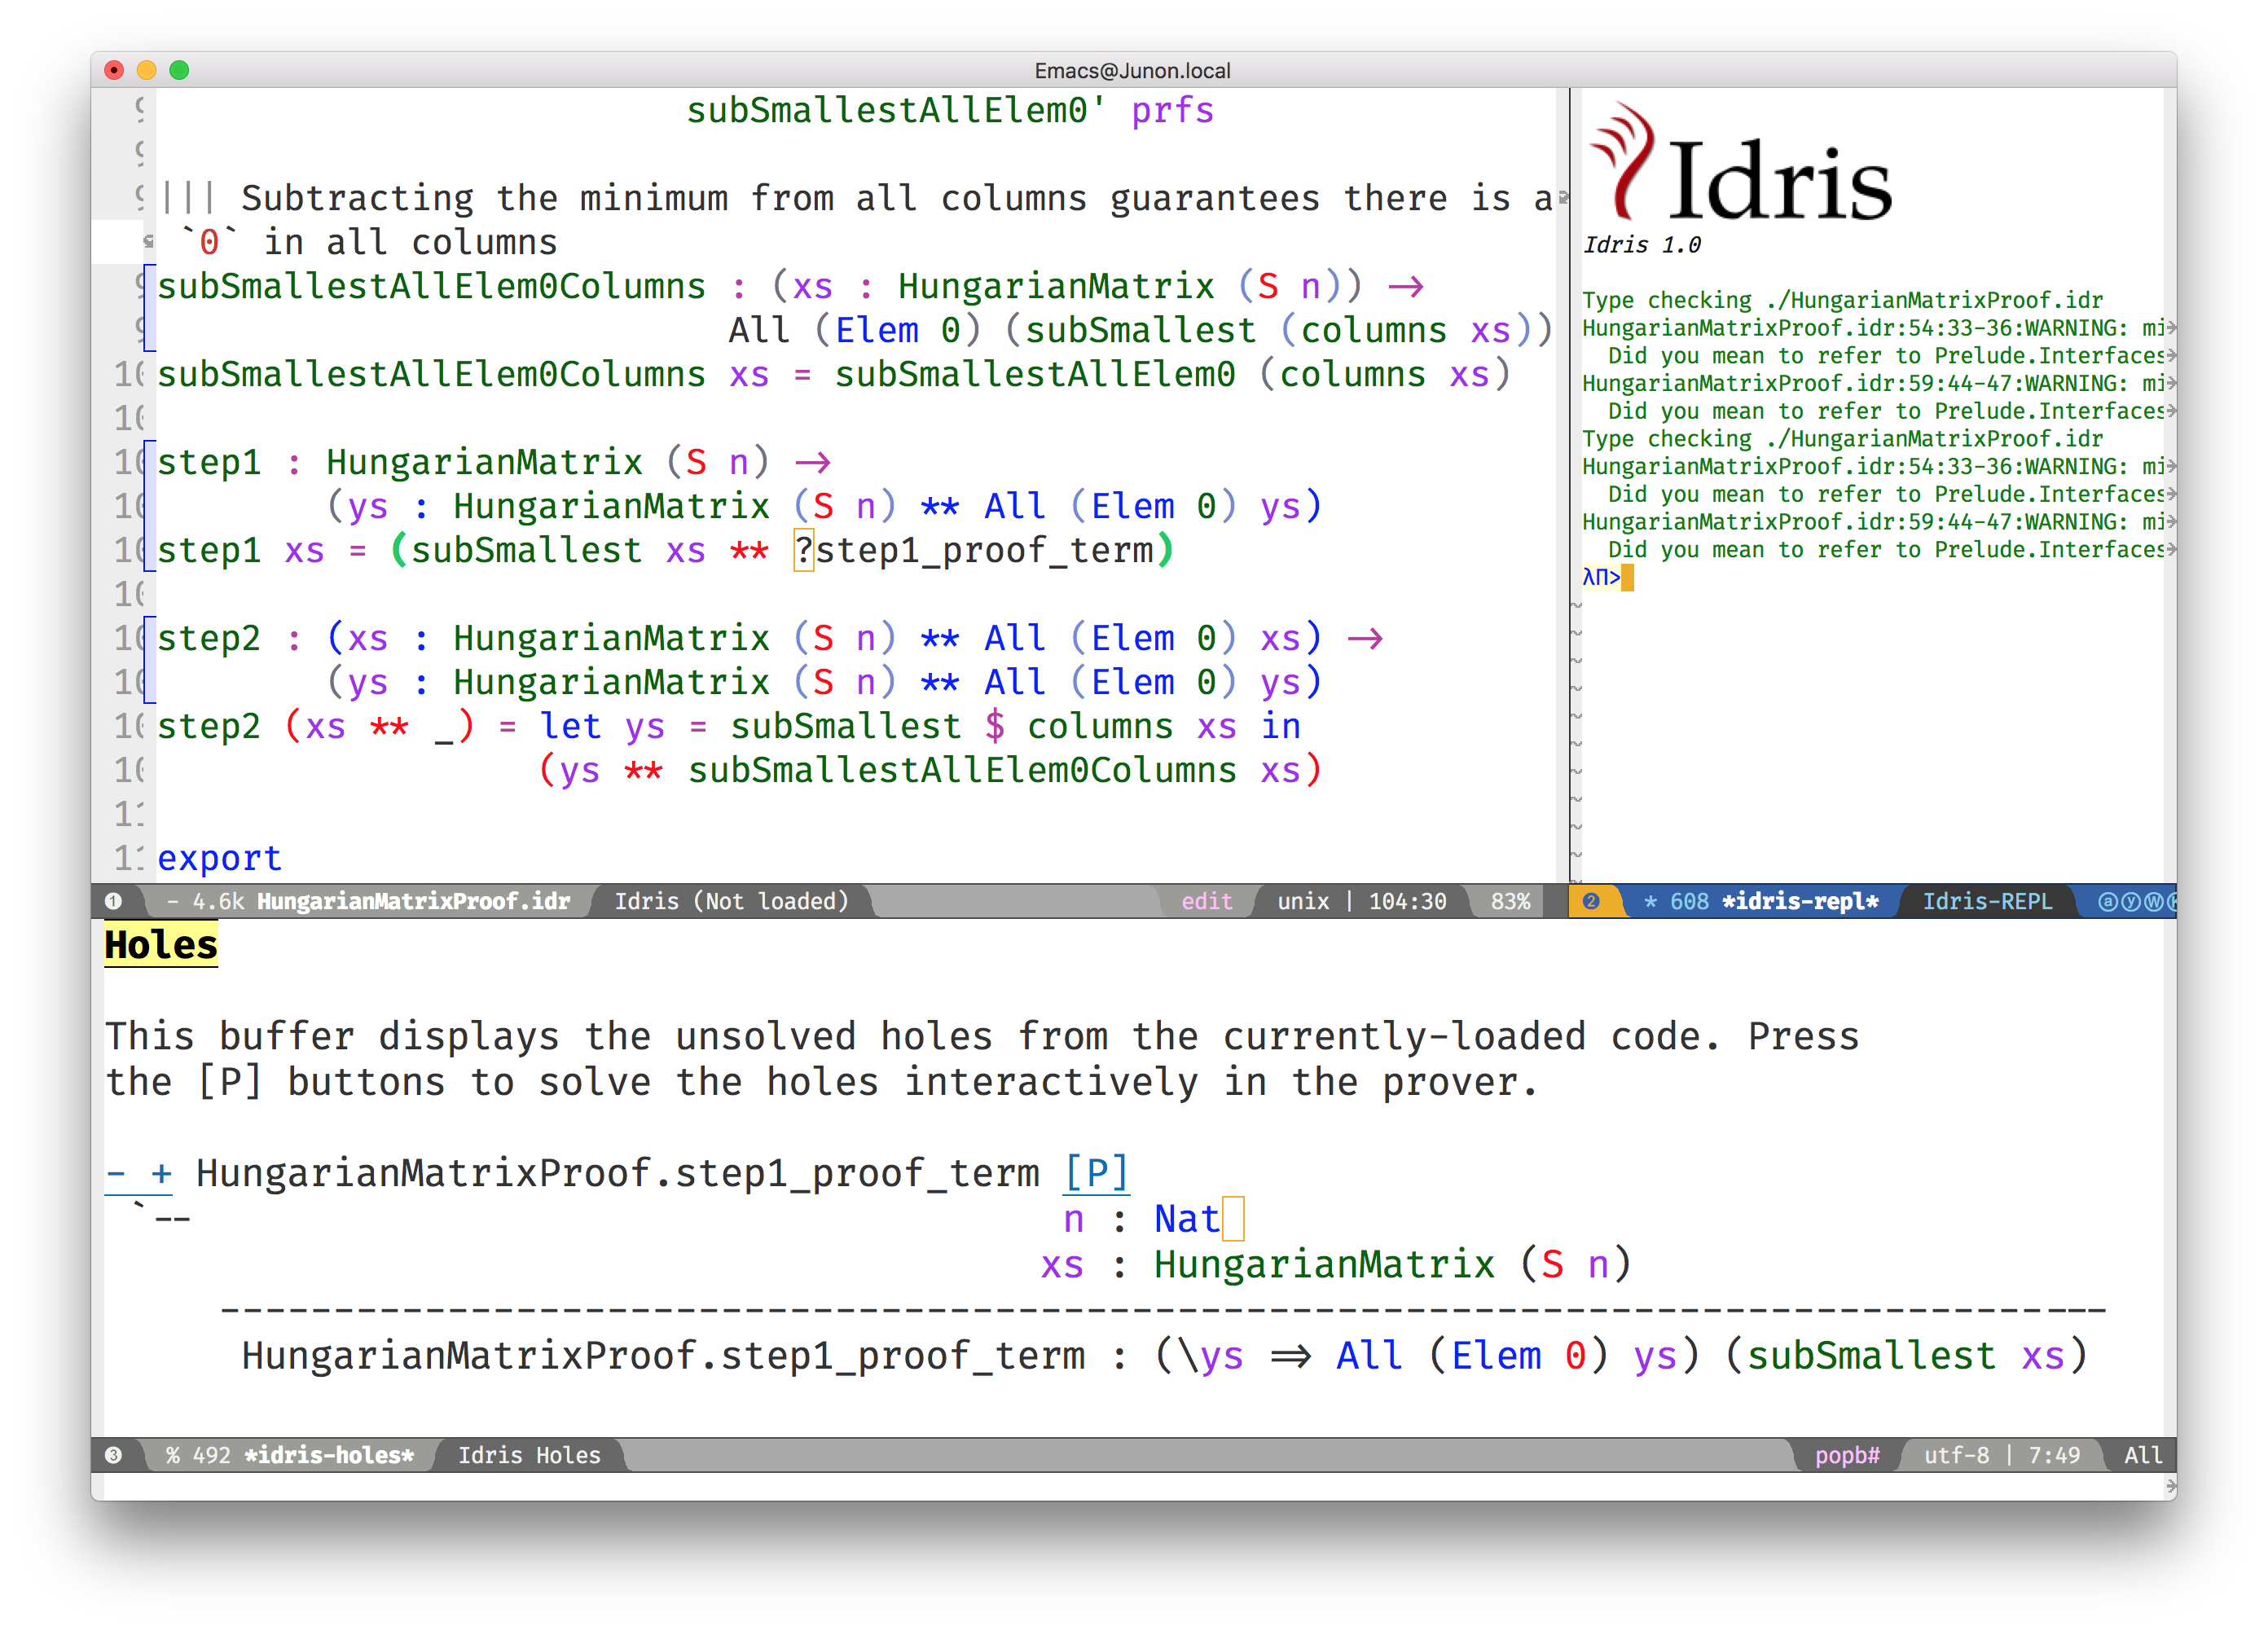
\includegraphics[width=0.85\linewidth]{./fig/interactive_idris.png}
\caption{An in-progress editing session using the interactive Idris mode}
\end{figure}

\section{Type-Driven Development}
\label{sec:org54d445b}
The type-driven development approach is an iterative system for building up a
definition of a function or a set of functions using dependent types. The
approach is outlined, advocated and used throughout Edwin Brady's book
\cite{brady_book_2017} on Idris and this style of development. The approach
consists of three main steps:
\begin{enumerate}
\item Type
\item Define
\item Refine
\end{enumerate}

The first step, ``Type'', tells us to create an initial specification of what
the function should do by writing down the type we want it to have. The approach
is top-down from the type through to the function clauses in the definition. The
type serves as a specification that will help guide us towards a correct
implementation.

In the second step, ``Define'', we create an initial definition for the
function, possibly leaving in some typed holes. We do not yet know exactly how
to make our definition line up with the specification in the type so we use
holes to defer the actual implementation of the function. At this point we
should make use of as much knowledge as we know to the point where we can't
continue to implement the function. We can gain more information by making use
of features such as case splitting. We may also refer back to step one and
modify the type to continue with the process.

The third step, ``Refine'', is where we complete the function definition,
possibly modifying the type. This is the point where we use the other
definitions and functions available in our environment to complete our
type-checked definition according to our specification. We may at this point
realise also that our initial specification was incorrect or missing some piece
of information so that can lead us back to our first step in the cycle and we
can continue from there with a more rigorous type specification to drive our
implementation from.

\begin{figure}[H]
\centering
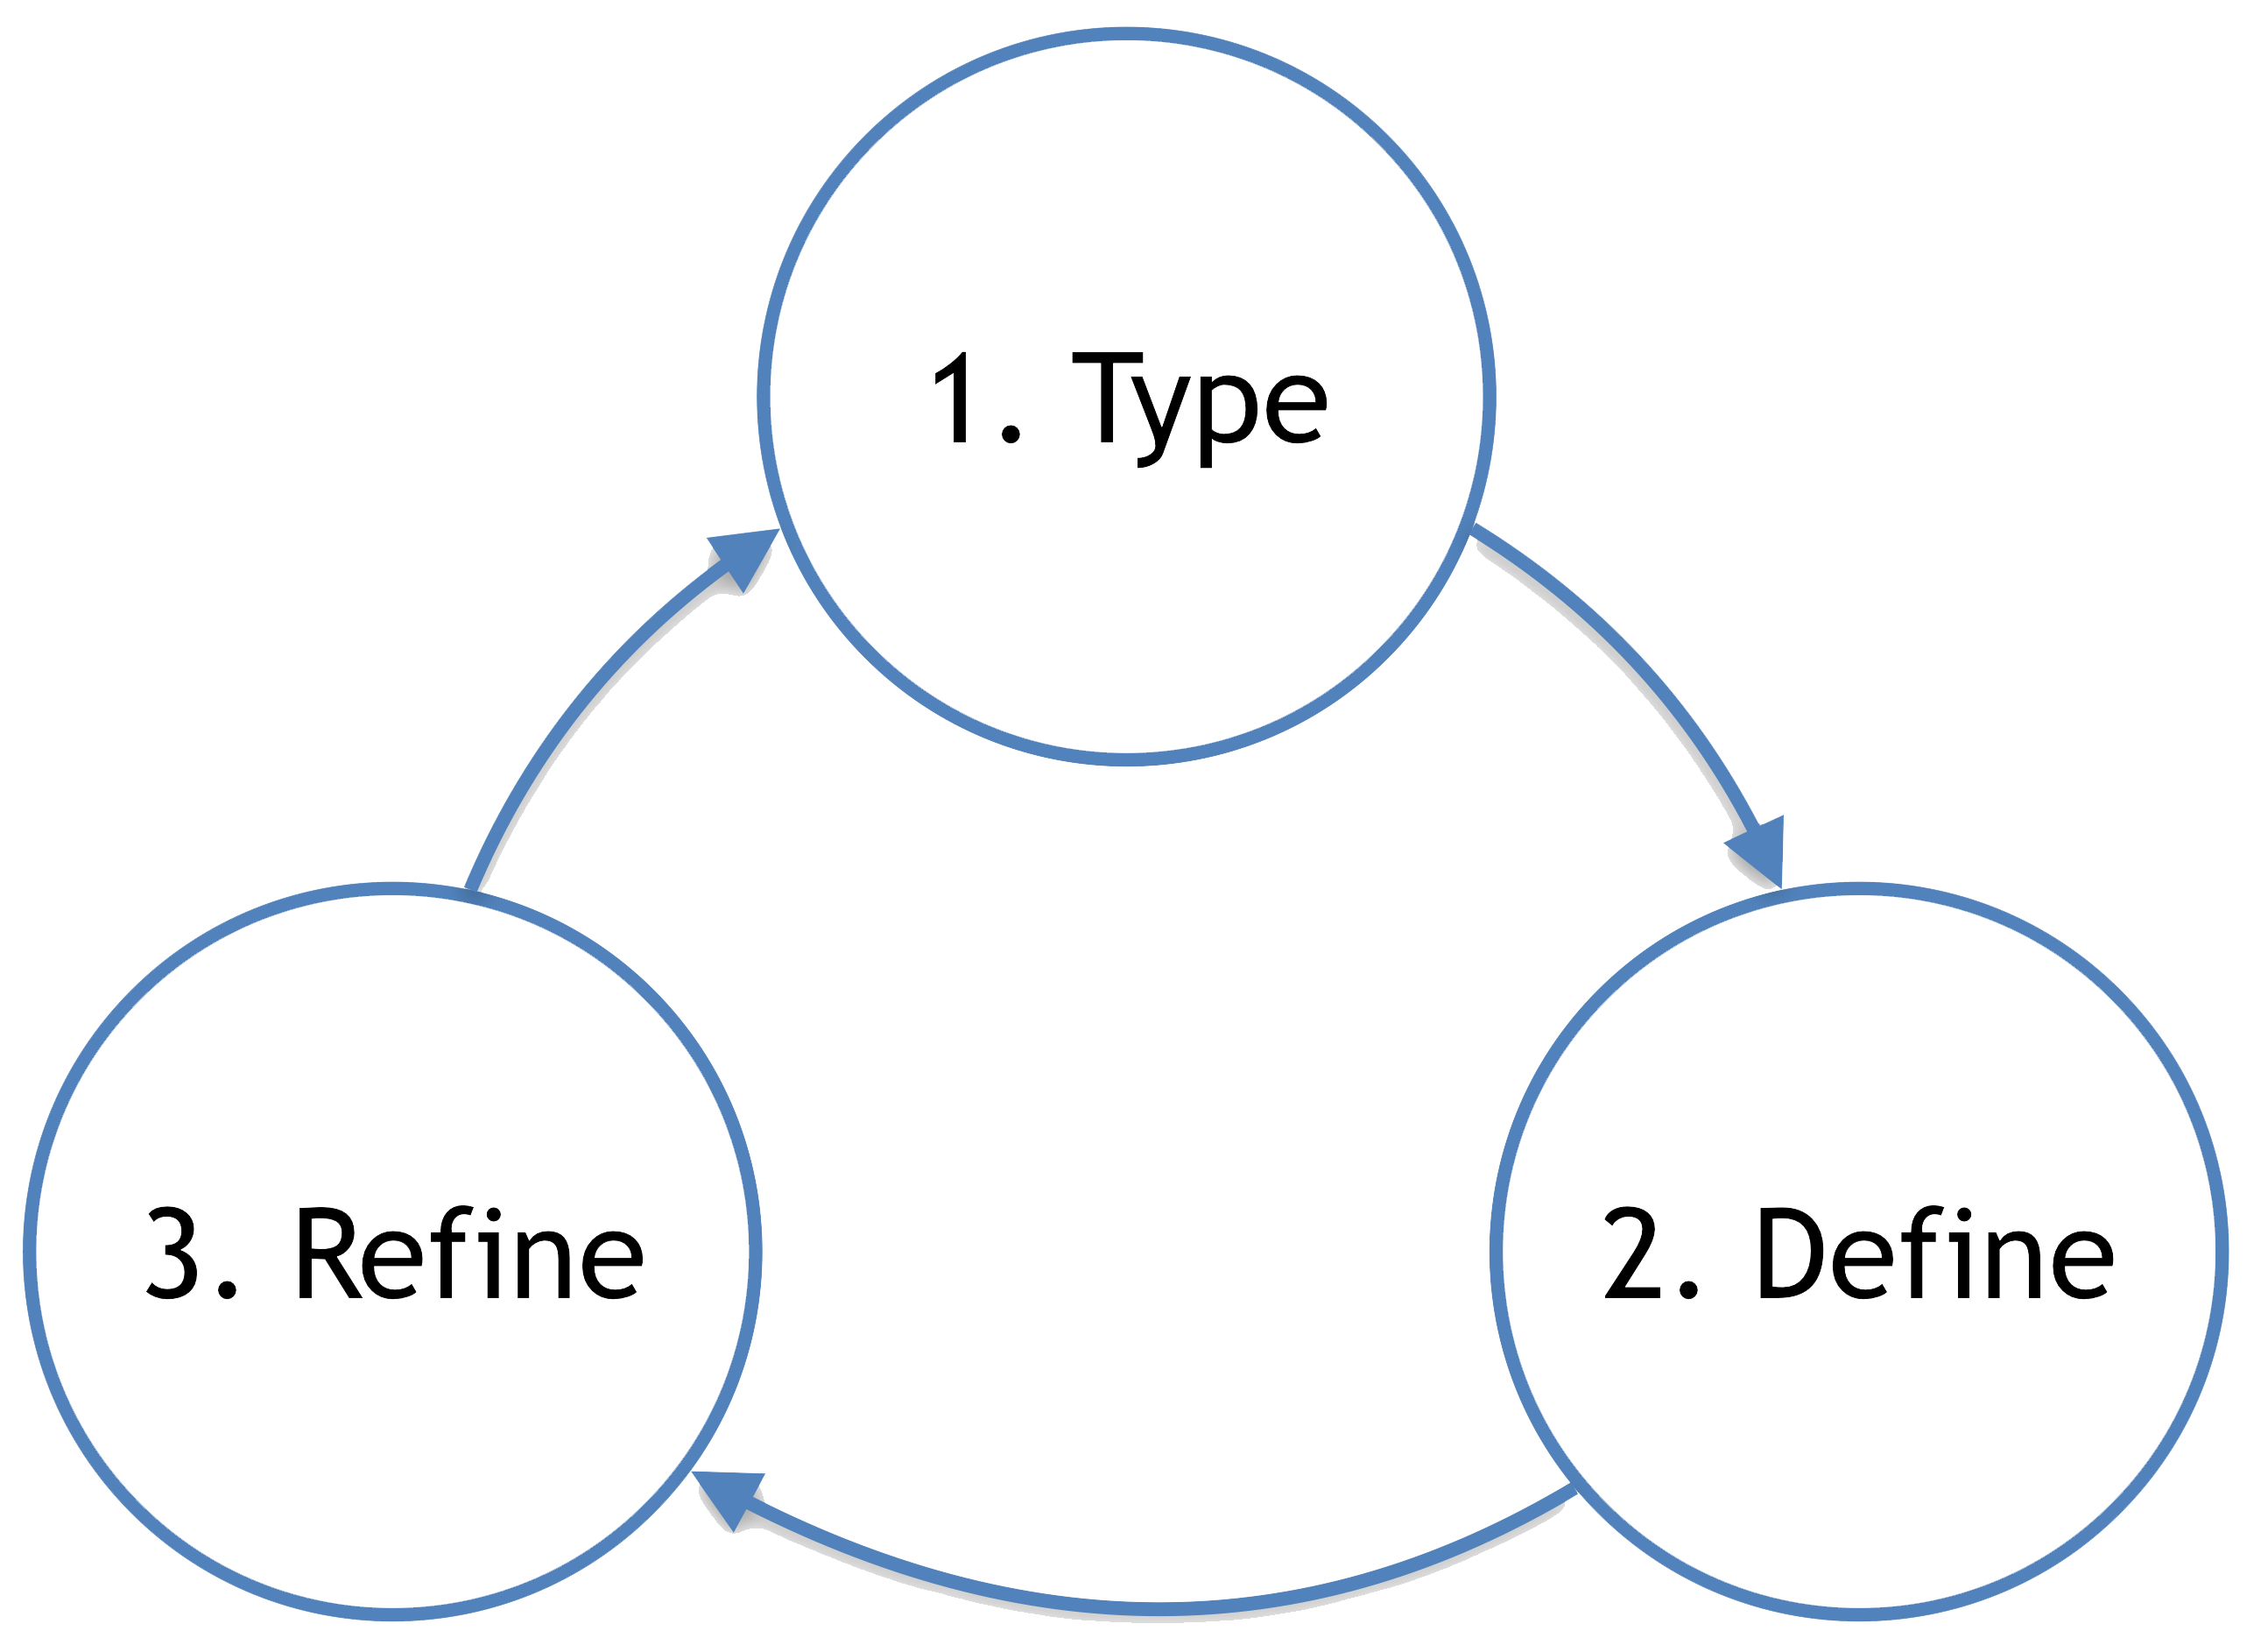
\includegraphics[width=0.8\linewidth]{./fig/tdd_cycle.png}
\caption{An illustration of the main workflow of the type-driven development approach}
\end{figure}

This style of development is greatly helped by the use of one of Idris'
interactive editing modes described earlier. In some cases the only manual
typing we might have to do is just writing our initial type specification. The
definition step in particular is aided. Using interactive editing modes we can
introduce an initial definition, case split on arguments and even try an initial
proof search on the typed holes we introduce. It may work out that the compiler
has everything it needs to create a correct type-checked definition without any
manual input from the user beyond the type of the function.

If we do need to provide more information, again, interactive editing helps get
us there. We can continue to inspect our environment to see the types of the
holes we need to define and also the environment of information available to us.
Reloading our modules and inspecting our current goals is one of the main
activities when programming in this type-driven fashion. As we continue to
refine our definition this type information also becomes refined and we can
continue to iterate over refining and modifying our types to reach a complete
definition.
\chapter{Case Studies}
\label{sec:org4d1a853}
\section{The Assignment Problem}
\label{sec:orga7510c7}
The first case study we'll examine is an implementation of a solution to the
assignment problem based off the Hungarian algorithm with correctness guarantees
maintained throughout the steps of the algorithm.

\subsection{Problem Definition}
\label{sec:orgf849204}
The assignment problem is a classic example of a combinatorial optimisation
problem. The problem involves assigning a number of \emph{agents} to \emph{tasks}. An agent
can be assigned to any task however there is a cost to assigning a particular
agent to a particular task. The assignment problem is the problem of assigning
exactly one task to each agent so that the total cost of doing this assignment
is minimal.

To think of the problem in a concrete setting we might imagine a clinical
practice with patients that need treatments as our tasks. The agents in this
scenario are the doctors that will be assigned to treat patients. Doctors can
perform the treatment for any of the patients but a doctor may be suited more
towards a specific kind of treatment. The assignment problem in this setting is
finding a way to assign the doctors to treat the patients in a way that
optimally assigns the doctors based on their ability to perform specific
treatments.

\subsection{Existing Algorithms}
\label{sec:orgc6fbbc8}
It may seem that the time complexity of an algorithm to solve such a problem
would require time in the order \(O(n!)\) time with respect to the number of
agents/tasks. Optimisation strategies exist however that produce polynomial time
algorithms. The most famous example is the Hungarian algorithm which runs in
\(O(n^4)\) time. Further algorithmic optimisations have been applied such as James
Munkres' proven algorithm \cite{munkres_assignment_1957} that demonstrates
\(O(n^3)\) time complexity.

\subsection{Hungarian Algorithm}
\label{sec:org073e792}
Our Idris implementation focuses on implementing the Hungarian algorithm due to
its straight forward specification. There are also a number of correctness
properties that jump off the page when reading the specification that we can
attempt to write proofs for and in turn create a verified implementation that
follows the steps properly. The Hungarian algorithm frames the problem in terms
of a matrix that represents the tasks, agents and the weighting between them.

The steps of the algorithm are as follows:
\begin{enumerate}
\item Find the minimum value in each row and subtract it from all other values in
its row.
\item Find the minimum value in each column and subtract it from all other values
in its column.
\item Cover each 0 in the matrix with a line such that the minimal number of lines
is used.
\item Find the smallest value in the cost matrix not covered by a line. Subtract it
from each uncovered row. Add it to each covered column. Return to step 3.
\end{enumerate}

We determine if we have completed an assignment following each step. For step 1
this means checking if there is a 0 in each column. For the steps after step 1
we check if we have created a minimal covering. If the minimum number of
covering lines required is equal to the size of our square matrix then a minimal
assignment has been found and the algorithm has been completed.

The approach taken in this case study was to provide three different versions of
the algorithm, each one providing more correctness guarantees than the previous.
In order to accomplish this within the time constraints of the project only the
first two steps of the algorithm are being considered. However there are
interesting correctness properties that we can discuss and also some interesting
design decisions made in terms of approach and design of our API.

\subsection{Demonstration}
\label{sec:org186bd32}
First let us assume that we have some initial matrix that describes our tasks
and our agents that we would like to create an assignment for.

\[ \begin{bmatrix}
8 & 20 & 12 \\
3 & 2 & 14 \\
9 & 8 & 4
\end{bmatrix} \]

When applying step 1 we choose 8 in the first row, 2 in the second row and 4 in
the last row. We then subtract these values across their respective rows. This
results in the transformed matrix below.

\[ \begin{bmatrix}
\textcolor{red}{8} & 20 & 12 \\
\textcolor{red}{2} & 3 & 14 \\
9 & 8 & \textcolor{red}{4}
\end{bmatrix} \rightarrow
\begin{bmatrix}
0 & 12 & 4 \\
0 & 1 & 12 \\
5 & 4 & 0
\end{bmatrix} \]

As we can see, there are zeroes in both the first and third columns but there is
not a zero in the second column. We have yet to create a minimal assignment so
we proceed to apply step 2 to the transformed matrix that resulted from applying
the first step.

\[ \begin{bmatrix}
\textcolor{red}{0} & 12 & 4 \\
0 & \textcolor{red}{1} & 12 \\
5 & 4 & \textcolor{red}{0}
\end{bmatrix} \rightarrow
\begin{bmatrix}
0 & 11 & 4 \\
0 & 0 & 12 \\
5 & 3 & 0
\end{bmatrix} \]

When we have completed step 2 we now create a set of lines that will cover all
of the zeroes in the matrix. As we can see we have had to draw a minimum of 3
lines to cover the zeroes in the matrix at this point.

\[
\stackinset{c}{}{c}{1.0\baselineskip}{\rule{2.8\baselineskip}{.5pt}}{%
\stackinset{c}{}{c}{0.01\baselineskip}{\rule{2.8\baselineskip}{.5pt}}{%
\stackinset{c}{1.05\baselineskip}{c}{}{\rule{.5pt}{2.7\baselineskip}}{%
\begin{bmatrix}
  0 & 11 & 4 \\
  0 & 0 & 12 \\
  5 & 3 & 0
\end{bmatrix}}}}
\]

We have created a minimal covering with the number of lines equal to the size of
our matrix. The algorithm tells us that we have found a minimal assignment at
this point and we can stop. In this case, the first agent is assigned task 1,
the second agent is assigned task 2 and the third agent is assigned task 3.

\subsection{Invariants}
\label{sec:orgcbe79e5}
There are some interesting invariants we notice when performing these steps.
After performing the first step we can be certain that at least one of the
values in each row will be a zero. The minimum value that we find must be an
element of the row. At some point when subtracting it across the row we will
subtract it from itself. This will result in at least one zero.

\textbf{Step 1}:
\begin{itemize}
\item Precondition - A non-empty matrix
\item Postcondition - A non-empty matrix where all rows contain at least one zero
\end{itemize}

Similarly we can say that after completing the second step there will be at
least one zero in each row and at least one zero in each column. This follows
from the same reasoning as before because the element we subtract from the
column will be an element of that column.

\textbf{Step 2}:
\begin{itemize}
\item Precondition - A non-empty matrix where all rows contain at least one zero
\item Postcondition - A non-empty matrix where all rows contain at least one zero
and all columns contain at least one zero
\end{itemize}

These invariants will be studied in more detail as we outline the development of
the different Idris implementations of the algorithm.

\subsection{First Implementation - Lists}
\label{sec:org1833106}
The first implementation uses the standard list type. As we will see, this
implementation demonstrates the fewest number of correctness guarantees with no
proofs of the invariants outlined given and introduces partiality and the risk
of runtime errors that come with partial functions. This implementation is quite
similar to how you might approach the problem in a language such as Haskell with
limited information at the type level.

In order to implement the algorithm we first need to decide how the data is
modelled. In this list implementation our matrix will be defined as a list of
lists of ints. We can use Idris' ability to calculate types as the results of
functions to create some type aliases that allow us to write more specific types
that relate to the domain of the algorithm. In this case, \texttt{HungarianMatrix} as
opposed to \texttt{List (List Int))}.

\begin{listing}[H]
\begin{minted}[frame=single,fontsize=\normalsize,linenos,breaklines,escapeinside=\#\#]{idris}
Matrix : Type -> Type
Matrix a = List (List a)

HungarianMatrix : Type
HungarianMatrix = Matrix Int
\end{minted}
\caption{Type aliases to represent our cost matrix}
\end{listing}

As both the first step and the second step of the algorithm require that we find
the minimum of rows and columns respectively we will need to define a function
that finds the minimum of a list that contains elements with some notion of ordering.

\begin{listing}[H]
\begin{minted}[frame=single,fontsize=\normalsize,linenos,breaklines,escapeinside=\#\#]{idris}
listMin' : Ord a => a -> List a -> a
listMin' x [] = x
listMin' x (y :: ys) with (compare x y)
  listMin' x (y :: ys) | GT = listMin' y ys
  listMin' x (y :: ys) | EQ = listMin' y ys
  listMin' x (y :: ys) | LT = listMin' x ys

partial
listMin : Ord a => List a -> a
listMin (x :: xs) = listMin' x xs
\end{minted}
\caption{The \texttt{minimum} function defined over lists}
\end{listing}

In this function we've made use of the interface mechanism of Idris. This system
is analogous to the type class system in Haskell. We can define the \texttt{listMin}
function using ad-hoc polymorphism over any type that provides an implementation
of the \texttt{Ord} interface.

Despite this function working as intended and type-checking, a problem is
starting to emerge. The \texttt{listMin} function is a partial function. There is no
minimum value that we can get from an empty list. If the provided matrix is
empty then we will receive an error at runtime and crash. The compiler has been
able to catch this function if we had left out the \texttt{partial} annotation due to the
use of the \texttt{\%default total} compiler pragma in our implementations.

One way we might solve this problem is by taking a default value as an extra
argument. This however does not make sense semantically as it is not the minimum
value of the passed list. We will have to accept when using lists that we may
have an empty case and as such our \texttt{listMin} function is partial.

The effect of this partial function at the centre of this implementation of the
algorithm is that it has a chain reaction on the totality of the rest of the
functions required to implement the algorithm. We now consider the effect of
this partiality on our \texttt{subSmallest} function that performs the step of
subtracting our minimum values across all rows/columns in our matrix.

\begin{listing}[H]
\begin{minted}[frame=single,fontsize=\normalsize,linenos,breaklines,escapeinside=\#\#]{idris}
partial
subSmallest : HungarianMatrix -> HungarianMatrix
subSmallest [] = []
subSmallest (x :: xs) = map (flip (-) $ (listMin x)) x :: subSmallest xs
\end{minted}
\caption{Subtracting the minimum values across the matrix}
\end{listing}

As defined, \texttt{subSmallest} matches both cases, the empty list case and the
non-empty case. Then we might ask why does this function have an annotation that
it is partial? The reason is that in the second function clause we make a call
to the \texttt{listMin} function. As this function is partial this has the knock-on
effect of introducing partiality into the \texttt{subSmallest} function which is used
throughout the algorithm. If we were to remove this partiality annotation the
compiler will correctly inform us that the function has failed to satisfy the
totality checker.

\begin{verbatim}
idris> :total subSmallest
HungarianList.subSmallest is possibly not total due to:
    HungarianList.listMin, which is not total as there are missing cases
\end{verbatim}

This partiality bubbles up to the top level of the algorithm at the point where
we export the function that end users will use. Any consumer of this algorithm
should be prepared to either ensure that they never provide an empty matrix to
the \texttt{hungarianMethod} function or they risk that their program crashes due to an
unmatched pattern in the \texttt{listMin} function.

Obviously we would like to do better than that and not introduce ways to crash
code calling into our algorithm. These kinds of errors should be caught
statically at compile time. Fortunately Idris provides the tools to ensure that
these kinds of errors are made impossible through sufficiently descriptive
types. This is the avenue we will explore and demonstrate with the next
implementation.

\subsection{Second Implementation - Vectors}
\label{sec:orgff86cdc}
In the second implementation we begin to narrow down the possibilities of
incorrect type-checking functions. To start off with, the definition of our
\texttt{HungarianMatrix} type has been modified. We make use of the Idris standard
library type \texttt{Matrix n m a} which is simply defined as \texttt{Vect n (Vect m a)}.

\begin{listing}[H]
\begin{minted}[frame=single,fontsize=\normalsize,linenos,breaklines,escapeinside=\#\#]{idris}
HungarianMatrix : (n : Nat) -> {auto p : n `GT` Z} -> Type
HungarianMatrix Z {p = LTEZero} impossible
HungarianMatrix Z {p = (LTESucc _)} impossible
HungarianMatrix (S k) {p = (LTESucc x)} = Matrix (S k) (S k) Int
\end{minted}
\caption{Type alias to represent our cost matrix}
\end{listing}

There are a couple of things worth noting in this definition. The aim of this
type alias is to ensure that our \texttt{HungarianMatrix} can only represent the square
matrices that have at least 1 row and column. The first argument to this
type-computing function is the size \(n\) of our matrix.

The second argument represents a proof that \(n > 0\). The curly braces
surrounding this argument denote that it is an implicit argument as outlined in
the previous chapter. As it is implicit, we do not need to explicitly pass this
proof when calling this function to create the type. For example, we can refer
to a square matrix of size 2 as having the type \texttt{HungarianMatrix (S (S Z))}
rather than \texttt{HungarianMatrix (S (S Z)) someProofTerm}. The use of the \texttt{auto}
keyword allows the compiler to perform a proof search to find the proof term
that fits instead of forcing us as the user to create it.

We can bring the implicit argument p down to our function definition and perform
a case split on it. We know that if the natural number passed to the function is
ever zero then it is impossible to have a value of type \texttt{Z `GT` Z} and as such
the compiler accepts that the two clauses above are impossible. This definition
was carried out in a type-driven way by defining our initial specification that
\(n\) had to be greater than zero (i.e. we wanted to create a non-empty matrix).
By using the interactive editing capabilities of Idris and case splitting on the
proof term, the clauses above fell out immediately leaving just one clause that
wasn't impossible and where we could insert the definition of our non-empty
matrix.

Using the \texttt{Vect} type of length-indexed lists helps us achieve more totality in
this implementation. In our previous list of lists based version the partiality
of our \texttt{listMin} function had the effect of bubbling up and creating partiality in
all of the functions in our interface. Using the \texttt{Vect} type of length-indexed
lists we can reduce the number of cases that need to be matched in order to
achieve a total definition of a minimum function. Restricting our type to only
work on vectors that have at least one element ensures that we can always return
a value from the \texttt{vectMin} function. If we tried to pattern match on the nil
constructor for \texttt{Vect} then that would result in a type error as we've explicitly
stated in the type of \texttt{vectMin} that it will only accept vectors with at least one
element as input.

\begin{listing}[H]
\begin{minted}[frame=single,fontsize=\normalsize,linenos,breaklines,escapeinside=\#\#]{idris}
vectMin' : Ord a => a -> Vect n a -> a
vectMin' x [] = x
vectMin' x (y :: ys) with (compare x y)
  vectMin' x (y :: ys) | GT = vectMin' y ys
  vectMin' x (y :: ys) | EQ = vectMin' y ys
  vectMin' x (y :: ys) | LT = vectMin' x ys

vectMin : Ord a => Vect (S n) a -> a
vectMin (x :: xs) = vectMin' x xs
\end{minted}
\caption{The \texttt{minimum} function defined over length-indexed lists}
\end{listing}

The effect that this has on our code is that now if a consumer of our algorithm
tries to call into it with an empty matrix that error can be statically detected
at compile time. We don't run the risk of introducing runtime errors that may
only be detected when a system has been running for days with buggy and
under-specified code. This reflects itself in the types of the functions that
implement the specific steps in the algorithm. The types outlined below provide
us with the knowledge that we can never call these functions with ill-typed data
such as empty matrices.

\begin{listing}[H]
\begin{minted}[frame=single,fontsize=\normalsize,linenos,breaklines,escapeinside=\#\#]{idris}
step1 : HungarianMatrix (S n) -> HungarianMatrix (S n)

step2 : HungarianMatrix (S n) -> HungarianMatrix (S n)

export
hungarianMethod : HungarianMatrix (S n) -> HungarianMatrix (S n)
\end{minted}
\caption{Types of the algorithm's steps}
\end{listing}

Although we have now introduced an implementation of the algorithm which passes
the Idris totality checker by encoding the size of our cost matrix in the type
we have yet to provide any meaningful correctness properties for the steps of
the algorithm. We would like to be able to reason about the algorithm in terms
of the invariants mentioned before.

\subsection{Third Implementation - Vectors with Proofs}
\label{sec:org61dccbe}
In the third implementation we will build upon the previous attempt using
vectors. In this implementation however, we will create proofs about the code
that we write and enforce the invariants discussed previously. If we want to be
more certain about the correctness of the code that we write we will need to be
able to construct correct proofs that type check but are also semantically
correct in that the type is a correct specification for the proof.

The invariants discussed previously have something in common. They both express
that there must exist a zero somewhere in our matrix. The Idris standard library
provides a type \texttt{Elem} which encodes exactly this notion of existence within a
vector. There are two constructors of this type, \texttt{Here} and \texttt{There}. \texttt{Here} represents
a proof that the element at the head of the vector is equal to the element that
is being shown to exist. The repeated use of the name \texttt{x} ensures that this
reflexive equality must hold in order to construct a \texttt{Here} value. \texttt{There}
represents the fact that if an item is an element somewhere later in the vector
then it is an element of a vector constructed by prepending an element to the
front of the vector in discussion.

\begin{listing}[H]
\begin{minted}[frame=single,fontsize=\normalsize,linenos,breaklines,escapeinside=\#\#]{idris}
||| A proof that some element is found in a vector
data Elem : a -> Vect k a -> Type where
     Here : Elem x (x::xs)
     There : (later : Elem x xs) -> Elem x (y::xs)
\end{minted}
\caption{The Idris standard library definition of \texttt{Elem}}
\end{listing}

This type allows us to express notions such as \texttt{(xs : Vect n a) -> Elem 0
(subSmallest xs)}. In our invariants however we want to encode that all of the
rows and columns contain a specific element. Idris also provides some
quantifiers that act over lists and vectors. These quantifiers \texttt{Any} and \texttt{All}
encode notions of existential quantification and universal quantification
respectively. If we look at how \texttt{All} is defined we can see that it is very
closely related to the \texttt{Vect} type we have been using. In a sense we can reason
about it as a vector of proofs that some property holds corresponding
element-wise to the \texttt{Vect} passed as an input to the type.

\begin{listing}[H]
\begin{minted}[frame=single,fontsize=\normalsize,linenos,breaklines,escapeinside=\#\#]{idris}
||| A proof that all elements of a vector satisfy a property. It is a list of
||| proofs, corresponding element-wise to the `Vect`.
data All : (P : a -> Type) -> Vect n a -> Type where
  Nil : {P : a -> Type} -> All P Nil
  (::) : {P : a -> Type} -> {xs : Vect n a} -> P x -> All P xs -> All P (x :: xs)
\end{minted}
\caption{The Idris standard library definition of \texttt{All}}
\end{listing}

We can implement a map-like operation that takes a vector and a function that
shows the property holds for any particular element of that vector and produce a
proof that the property holds for all elements of that vector.

\begin{listing}[H]
\begin{minted}[frame=single,fontsize=\normalsize,linenos,breaklines,escapeinside=\#\#]{idris}
proofMap : {P : a -> Type} -> ((x : a) -> P x) -> (xs : Vect n a) -> All P xs
proofMap _ [] = []
proofMap f (x :: xs) = f x :: proofMap f xs
\end{minted}
\caption{A proof mapping function to create a proof of \texttt{All}}
\end{listing}

Having looked at \texttt{Elem}, \texttt{All} and discussed some ways of creating proofs over
vectors and matrices we can now encode the invariants we outlined previously as
Idris types.

\begin{listing}[H]
\begin{minted}[frame=single,fontsize=\normalsize,linenos,breaklines,escapeinside=\#\#]{idris}
step1 : HungarianMatrix (S n) -> (ys : HungarianMatrix (S n) ** All (Elem 0) ys)

step2 : (xs : HungarianMatrix (S n) ** All (Elem 0) xs)
     -> (ys : HungarianMatrix (S n) ** All (Elem 0) ys)
\end{minted}
\caption{An encoding of our invariants as Idris types}
\end{listing}

The \texttt{step1} function says that we will take some non-empty matrix and produce not
only a transformed matrix after having performed the operations of the algorithm
but also a proof that all of the rows of this matrix contain a zero somewhere in
them. The \texttt{step2} function takes the result of the \texttt{step1} function and produces a
newly transformed matrix and also a proof that the columns of this new matrix
all contain a zero. In both of these functions we make use of the dependent pair
type, \texttt{**}. This is Idris' encoding of Martin-Löf's \(\Sigma\)-types. In both of these
examples the \emph{type} of the second element of the pair is dependent upon the \emph{value}
of the first.

We have also encoded some sense of ordering of the steps of the algorithm in
these types. We do not want to write correct implementations of the steps of the
algorithm and then interleave them in an incorrect order. By enforcing in step 2
that we first have a value that is of the type output from step 1 then we can
enforce an ordering between the steps of the algorithm. There should be no way
to call into step 2 without having obtained the value from having called step 1.
We can also think of this in terms of preconditions and postconditions. The
precondition of step 2 of the algorithm is the same as the postcondition of
step 1. This can continue for the other steps of the algorithm to ensure a
correct order of application.

There are a number of underlying proof steps that are required to get to the
point where we can write the functions \texttt{step1} and \texttt{step2} above.
\begin{enumerate}
\item The \texttt{vectMin} function produces a value present in the passed vector
\item Subtracting that value across a row/column produces at least one zero
\item Subtracting minimums across all rows/columns produces zeroes in all
rows/columns
\end{enumerate}

We will focus on this first proof step as an example to illustrate the approach
to performing these proofs in the type-driven style.

\begin{listing}[H]
\begin{minted}[frame=single,fontsize=\normalsize,linenos,breaklines,escapeinside=\#\#]{idris}
||| If we have a function to show `x` being in `zs` implies `x` being in `as`
||| and we can show `x` is in `y :: zs` then we can show `x` is in `y :: as`
congElem : (Elem x zs -> Elem x as) -> Elem x (y :: zs) -> Elem x (y :: as)
congElem _ Here = Here
congElem f (There later) = There (f later)

vectMinElem' : Ord a => (x : a) -> (ys : Vect n a) -> Elem (vectMin' x ys) (x :: ys)
vectMinElem' x [] = Here
vectMinElem' x (y :: ys) with (compare x y)
  vectMinElem' x (y :: ys) | GT = There (vectMinElem' y ys)
  vectMinElem' x (y :: ys) | EQ = There (vectMinElem' y ys)
  vectMinElem' x (y :: ys) | LT = congElem There (vectMinElem' x ys)

vectMinElem : Ord a => (xs : Vect (S n) a) -> Elem (vectMin xs) xs
vectMinElem (x :: xs) = vectMinElem' x xs
\end{minted}
\caption{Proof that \texttt{vectMin} produces an element of the passed vector}
\end{listing}

Structurally, this proof is very similar to the definitions of \texttt{vectMin} and
\texttt{vectMin'} discussed in the previous section. We can see that the proof is
deferred to a helper function \texttt{vectMinElem'} which states that if we have value \texttt{x}
and a vector \texttt{ys} then we can prove that applying the helper function \texttt{vectMin'} to
those arguments results in a value in \texttt{x :: ys}. For the empty vector, type-driven
development allows the compiler to know that the only case that is possible is
that the element must be at the current position as we have the singleton list
\texttt{[x]} in our type. In this case proof search is sufficient to find the correct
value for us.

The use of the \texttt{with} pattern for a non-empty vector allows us to dependently
pattern match on the result of the comparison. If the value at the head of the
vector is either greater than or equal to the current minimum, by the definition
of the \texttt{vectMin'} function, we know that the value returned will not be \texttt{x} but some
later value and so the constructor \texttt{There} is used with a recursive call to
\texttt{vectMinElem'}. The \texttt{congElem} function represents the congruence of \texttt{Elem} in that if
we have an implication that \texttt{x} is in \texttt{zs} implies \texttt{x} being in \texttt{as} then if \texttt{x} is in \texttt{y
:: zs} that will imply that \texttt{x} is in \texttt{y :: as}. We use this to prove that our
minimum is in the vector when it continues to be the minimum value inspected so
far while recursing through the vector. This gives a flavour of the approach
used when writing proofs of functions in Idris. The rest of the proofs for the
steps of the algorithm are provided as part of the full code listing for the
\texttt{HungarianMatrixProof} module should you wish to inspect more of these same
approaches at work.

There were some particular challenges that appeared while writing this
implementation. The first of which was the lack of dependent pattern matching
for integers. As \texttt{Int} is defined as a primitive type in Idris we cannot perform
any meaningful induction over its structure like we can do with the \texttt{Nat}
datatype. As part of this proven implementation we need to be able to show that
subtracting a number from itself produces zero. If our implementation were using
natural numbers then we could leverage the already defined proof of this fact
from the standard library. Unfortunately the Hungarian algorithm has to deal
with negative numbers in the later steps of the algorithm and use of \texttt{Nat} won't
be satisfactory for an implementation. As we can't do dependent pattern matching
on \texttt{Int} we have to define this is a postulate that we tell Idris to trust. For
small and self-evident theorems such as this it may be acceptable to write a
postulate but we would like to encode as much of our proof within the Idris
framework as possible so having to use postulates is indicative of a problem in
the code. There exists a wrapper around \texttt{Nat} to represent signed integers in the
standard library however it was only discovered after the version using integers
was complete.

\begin{listing}[H]
\begin{minted}[frame=single,fontsize=\normalsize,linenos,breaklines,escapeinside=\#\#]{idris}
postulate minusSelfZero : {x : Int} -> x - x = 0
\end{minted}
\caption{We tell Idris to trust us that \(x\mathbin{-} x \mathrel{=} 0\)}
\end{listing}

Another pain point encountered were the sometimes complex type errors. In one
instance a particularly wordy and incomprehensible 200 line type error was
produced when attempting to prove that all of the rows contained zeroes. The use
of the names \texttt{meth1}, \texttt{meth5} etc. indicated that we needed to somehow examine how
interfaces were being used in our implementation. The problem turned out to only
demonstrate itself in a particular use of the \texttt{map} function from the \texttt{Functor}
interface. Replacing the call to \texttt{map} with a local definition specialised only to
work over \texttt{Vect} caused the type errors to disappear. This turned out to be a bug
in the Idris compiler and how it handles interfaces that has since been
corrected although we weren't aware of this at the time of writing the code.
These cryptic error messages can often manifest themselves when working in a
system with such an expressive type system. It will often be hard to tell if the
error is due to a mistake on your part or if it is some detail of a bug in the
compiler leaking out into your code.

\subsection{API Considerations}
\label{sec:orgbd8f65e}
It is worth considering what kind of API we wish to expose to the consumers of
our algorithm. Although we have these complicated proof terms as part of our
module we can make some decisions about how simple or complicated the API is to
use. In each implementation we have elected to export a simple function that
performs the steps of the algorithm. Each of our modules contains a definition
similar to the following.

\begin{listing}[H]
\begin{minted}[frame=single,fontsize=\normalsize,linenos,breaklines,escapeinside=\#\#]{idris}
export
hungarianMethod : HungarianMatrix (S n) -> HungarianMatrix (S n)
hungarianMethod xs = transpose (fst (step2 (step1 xs)))
\end{minted}
\caption{Our user-facing API for the Hungarian algorithm}
\end{listing}

With dependent types we can choose to expose as much or as little of the
underlying proof terms as we wish. We may not wish to complicate the use of our
library with the correctness proofs that ensure that we have a rigorous
implementation that is formally verified. We can achieve a simple user-facing
API while still having that formalism beneath ensuring that more static errors
are detected at compile time. To compliment this simple API a number of other
correctness proofs about the main functions could be exported from the module
separately. If someone wanted to take advantage of the fact the implementation
has been verified then they can use these properties in their code. For most
consumers of the library this will probably not be the case but it is still
possible to satisfy both the users that want a simple API and those that would
like access to the underlying formalism that ensures that the simple API behaves
as it should.

\subsection{Haskell Port - Bottom Up Approach}
\label{sec:org0fce2a2}
Another implementation approach taken when tackling this algorithm was to take
an existing Haskell version of the Hungarian method and port it to Idris. From
there, we could add further specification of the correctness of our
implementation to the types of the ported functions. This can be seen as more of
a bottom-up approach as compared to the top-down approach of type-driven
development where the specification (types) come first.

The code being ported was a package \cite{komuves_munkres_2008} on the Haskell
package server Hackage. The aim was to take this package and directly port the
code over to Idris however there were a number of complications with this
approach. The major problem was the use of efficient stateful data structures
such as \texttt{Data.Array} in the Haskell package. Idris doesn't provide an analogous
data structure to this efficient array type. The Haskell implementation had to
be pulled apart in order to translate it into a representation using lists and
recursion rather than mutating references to arrays. The surface syntax may make
it seem simple to port this code to Idris however that wasn't the case as we
found. There were some subtleties involved in getting the code to type-check in
Idris.

At this point we can begin to add our correctness proofs onto our ported Idris
code. Ultimately this work had to be abandoned and a new approach taken in the
type-driven style. The implementation wasn't suited to writing proofs at least
not in a simple manner. Much more benefit and success was had when writing code
that was specifically set out to be proven in the first place. This means
specifying the properties you want to prove at the outset in your types and by
implementing the functions in a type-driven development fashion.

\section{Run-Length Encoding}
\label{sec:orgadd8631}
The next case study we'll examine is an Idris implementation of run-length
encoding.

\subsection{Problem Definition}
\label{sec:org0523564}
Numerous compression algorithms and techniques exist to squeeze data into
occupying fewer bytes in memory or on disk. Often these algorithms optimise for
specific use cases. For example, the compression present in the JPEG image
format is lossy to because of the visual nature of the data being compressed.
Even with mild loss to the quality of the image the overall image will still be
only slightly distinguishable from the original image. Lossy compression schemes
also exist for audio and video data again to optimise data that is tolerant to a
loss of quality. For text however we don't want to introduce lossy compression
as that would distort the original meaning of the data perceivably.

Run-length encoding is a simple technique used to compress text data. The data
is encoded as a series of ``runs'' which represent multiple repeated occurrences
of a single character. To illustrate the working of this compression scheme the
string ``foooobaaaar'' would be encoded as ``1f4o1b4a1r''. There is one 'f'
followed by four 'o's and so on. If we were to store the run counters in 8 bit
unsigned integers and deal with 8 bit ASCII characters the compressed version
would come in at 10 bytes versus the original 11 bytes. This algorithm has saved
very little memory in this example but we can see how this might scale up for
longer runs in larger strings.

\subsection{Invariants}
\label{sec:orgdc7d0a6}
There are two invariants that we might want to prove about a compression scheme
such as run-length encoding. The first of which is that the compression
algorithm actually produces a value which occupies less space than the original
value. The second invariant is that there exists an identity from composing
compress and decompress. If we take some data and call a compression function on
it and then pass that result on to a decompression function then we would expect
to get back the same initial data that we compressed. In this sense \texttt{decompress
(compress data)} should be equal to \texttt{id data} and as a result \texttt{decompress . compress}
should equal \texttt{id}. For reasons outlined later we will see why both of these
invariants are either quite difficult or impossible to encode and prove.

\subsection{Idris Implementation}
\label{sec:org1f95c3d}
This case study began by taking an initial piece of example code from the Idris
repository that performed a simple run-length encoding. The initial code
demonstrated how a run-length encoder might be written but did not properly
encode the data. The output of the function was a string which does not
accurately represent how we want to encode the data. A proper encoder would
alternate between an 8 bit integer and an 8 bit ASCII character to produce an
efficient format capable of being written byte-by-byte to a file.

\begin{listing}[H]
\begin{minted}[frame=single,fontsize=\normalsize,linenos,breaklines,escapeinside=\#\#]{idris}
intermediate : {auto p : m `LTE` (S n)} -> Vect (S n) Char -> (m : Nat ** Vect (S m) (Nat, Char))
intermediate xs with (rle xs)
  intermediate (_ :: _) | REnd impossible
  intermediate (c :: (replicate n c ++ [])) | (RChar n c rs) = (_ ** [(S n, c)])
  intermediate (c :: (replicate n c ++ (z :: zs))) | (RChar n c rs)
    = let (_ ** ws) = intermediate (z :: zs)
        in (_ ** (S n, c) :: ws)
\end{minted}
\caption{Intermediate format encoder for run-length encoding}
\end{listing}

This function creates an intermediate representation of our run-length encoded
data as a vector of pairs of natural numbers and characters. The natural numbers
give the length of the run and the character represents the character that is
being counted for that run. As seen before, we make use of the dependent pair
type \texttt{**} to specify the length of our resultant vector. We also make use of \texttt{auto}
proof search to ensure that the length of the resultant vector is less than or
equal to the length of the vector of characters passed in to be compressed. This
should be the case as if we have all length 1 runs then the vectors will have
equal length and if there is ever a run that is more than 1 long then there will
be fewer intermediate values as we only need to store the character once with
its run length.

With our intermediate value representation we can now begin to turn the data
into bytes that are suitable for output to a file. Idris includes a library
\texttt{Data.Bits} that contains numerous functions for manipulating binary data. We can
represent the data that we want to flush out to our file as a list of \texttt{Bits 8}
values which essentially map down to bytes. The drawback of this approach is
that we will truncate runs longer than 255 as we only have 8 bits to work with.
An extension to this scheme could be added such that runs longer than 255 are
represented as separate runs.

\begin{listing}[H]
\begin{minted}[frame=single,fontsize=\normalsize,linenos,breaklines,escapeinside=\#\#]{idris}
compressedBits : (n : Nat ** Vect (S n) (Nat, Char)) -> List (Bits 8)
compressedBits (Z ** ((n, c) :: [])) = [intToBits (cast n), intToBits (cast (ord c))]
compressedBits ((S x) ** ((n, c) :: xs)) = intToBits (cast n) :: intToBits (cast (ord c)) :: compressedBits (x ** xs)
\end{minted}
\caption{Translation of our intermediate data to bytes}
\end{listing}

With the information encoded as bytes we can use the Idris \texttt{Data.Buffer} module to
allocate a buffer that we can write the data into. We know that the size of the
buffer we want to allocate will be 2 times the length of our intermediate vector
format. One byte will be allocated for the length of the run and one byte
allocated for the actual character. Recursion over our list of bytes allows us
to build up a series of \texttt{IO} actions for writing out to our allocated buffer. We
can then sequence these actions to perform the modifications to the buffer and
flush it out to a file as compressed data.

\begin{listing}[H]
\begin{minted}[frame=single,fontsize=\normalsize,linenos,breaklines,escapeinside=\#\#]{idris}
writeCompressed' : List (Bits 8) -> Buffer -> Int -> List (IO ())
writeCompressed' [] buf loc = [pure ()]
writeCompressed' ((MkBits x) :: xs) buf loc = setByte buf loc x :: writeCompressed' xs buf (loc + 1)

writeCompressed : List (Bits 8) -> Buffer -> List (IO ())
writeCompressed xs buf = writeCompressed' xs buf 0

main : IO ()
main = do
  putStrLn ("Compressing: " ++ testString)
  putStrLn $ show compressed
  let bufferSize = cast $ 2 * (S (fst inter))
  Just buffer <- newBuffer bufferSize
    | Nothing => putStrLn "Failed to allocate buffer" -- If out of memory
  sequence_ $ writeCompressed compressed buffer -- Fill buffer
  Right file <- openFile "output.bin" WriteTruncate -- Get file handle
    | Left _ => putStrLn "Failed to get file handle"
  writeBufferToFile file buffer bufferSize
  putStrLn "Output written to output.bin"
\end{minted}
\caption{The main RLE program}
\end{listing}

\subsection{Proving Our Invariants}
\label{sec:org7229e5b}
\chapter{Assessments and Conclusions}
\label{sec:orga161e83}
\chapter{Future Work}
\label{sec:orgd53dfd4}

\emergencystretch=1em
\printbibliography[heading=bibintoc, title=References]
\appendix
\end{document}